\documentclass[envcountsect,dvips]{beamer}

\setbeamertemplate{background canvas}[vertical shading][bottom=yellow!20,top=blue!10]
%\usetheme{Darmstadt}
\usetheme{Warsaw}
%\usefonttheme[onlysmall]{structurebold}

\usepackage{natbib}
\usepackage{bibentry}
\bibliographystyle{plain}
\usepackage{chngcntr}

\usepackage[utf8]{inputenc}
\usepackage{default}
\usepackage{amsmath}
\usepackage{amsfonts}
\usepackage{amssymb}

\usepackage{graphicx}
\usepackage{caption}
\usepackage{subcaption}

\usepackage{color,xcolor,ucs}% para textcolor

\usepackage{verbatim}

\newenvironment<>{varblock}[2][.9\textwidth]{%
  \setlength{\textwidth}{#1}
  \begin{actionenv}#3%
    \def\insertblocktitle{#2}%
    \par%
    \usebeamertemplate{block begin}}
  {\par%
    \usebeamertemplate{block end}%
  \end{actionenv}}

%%%%%%%%%%%%%%%%%%%%%%%%%%%%%%%%%%%%%%%%%%%%%%%%%%%%%%%%%%%%%%%%%%%%%%%%%%
\begin{document}

\title[Conversão A-D e D-A:   ] % (optional, only for long titles)
{Conversão AD e DA}
\subtitle{analogico-digital e digital-analogico}
\author[Fernando] % (optional, for multiple authors)
{Fernando Pujaico Rivera\inst{1}}
\institute[Universidade Federal de Lavras] % (optional)
{
  \inst{1}%
  Universidade Federal de Lavras
}
\date[2016] % (optional)
{Aula-1 2016}
\subject{Computer Science}
\frame{\titlepage}

%%%%%%%%%%%%%%%%%%%%%%%%%%%%%%%%%%%%%%%%%%%%%%%%%%%%%%%%%%%%%%%%%%%%%%%%%%%%%%%%
%%%%%%%%%%%%%%%%%%%%%%%%%%%%%%%%%%%%%%%%%%%%%%%%%%%%%%%%%%%%%%%%%%%%%%%%%%%%%%%%
%%%%%%%%%%%%%%%%%%%%%%%%%%%%%%%%%%%%%%%%%%%%%%%%%%%%%%%%%%%%%%%%%%%%%%%%%%%%%%%%
\section{Conversão}

%%%%%%%%%%%%%%%%%%%%%%%%%%%%%%%%%%%%%%%%%%%%%%%%%%%%%%%%%%%%%%%%%%%%%%%%%%%%%%%%
\begin{frame}{Conversão entre digital e analógico }
\begin{center}
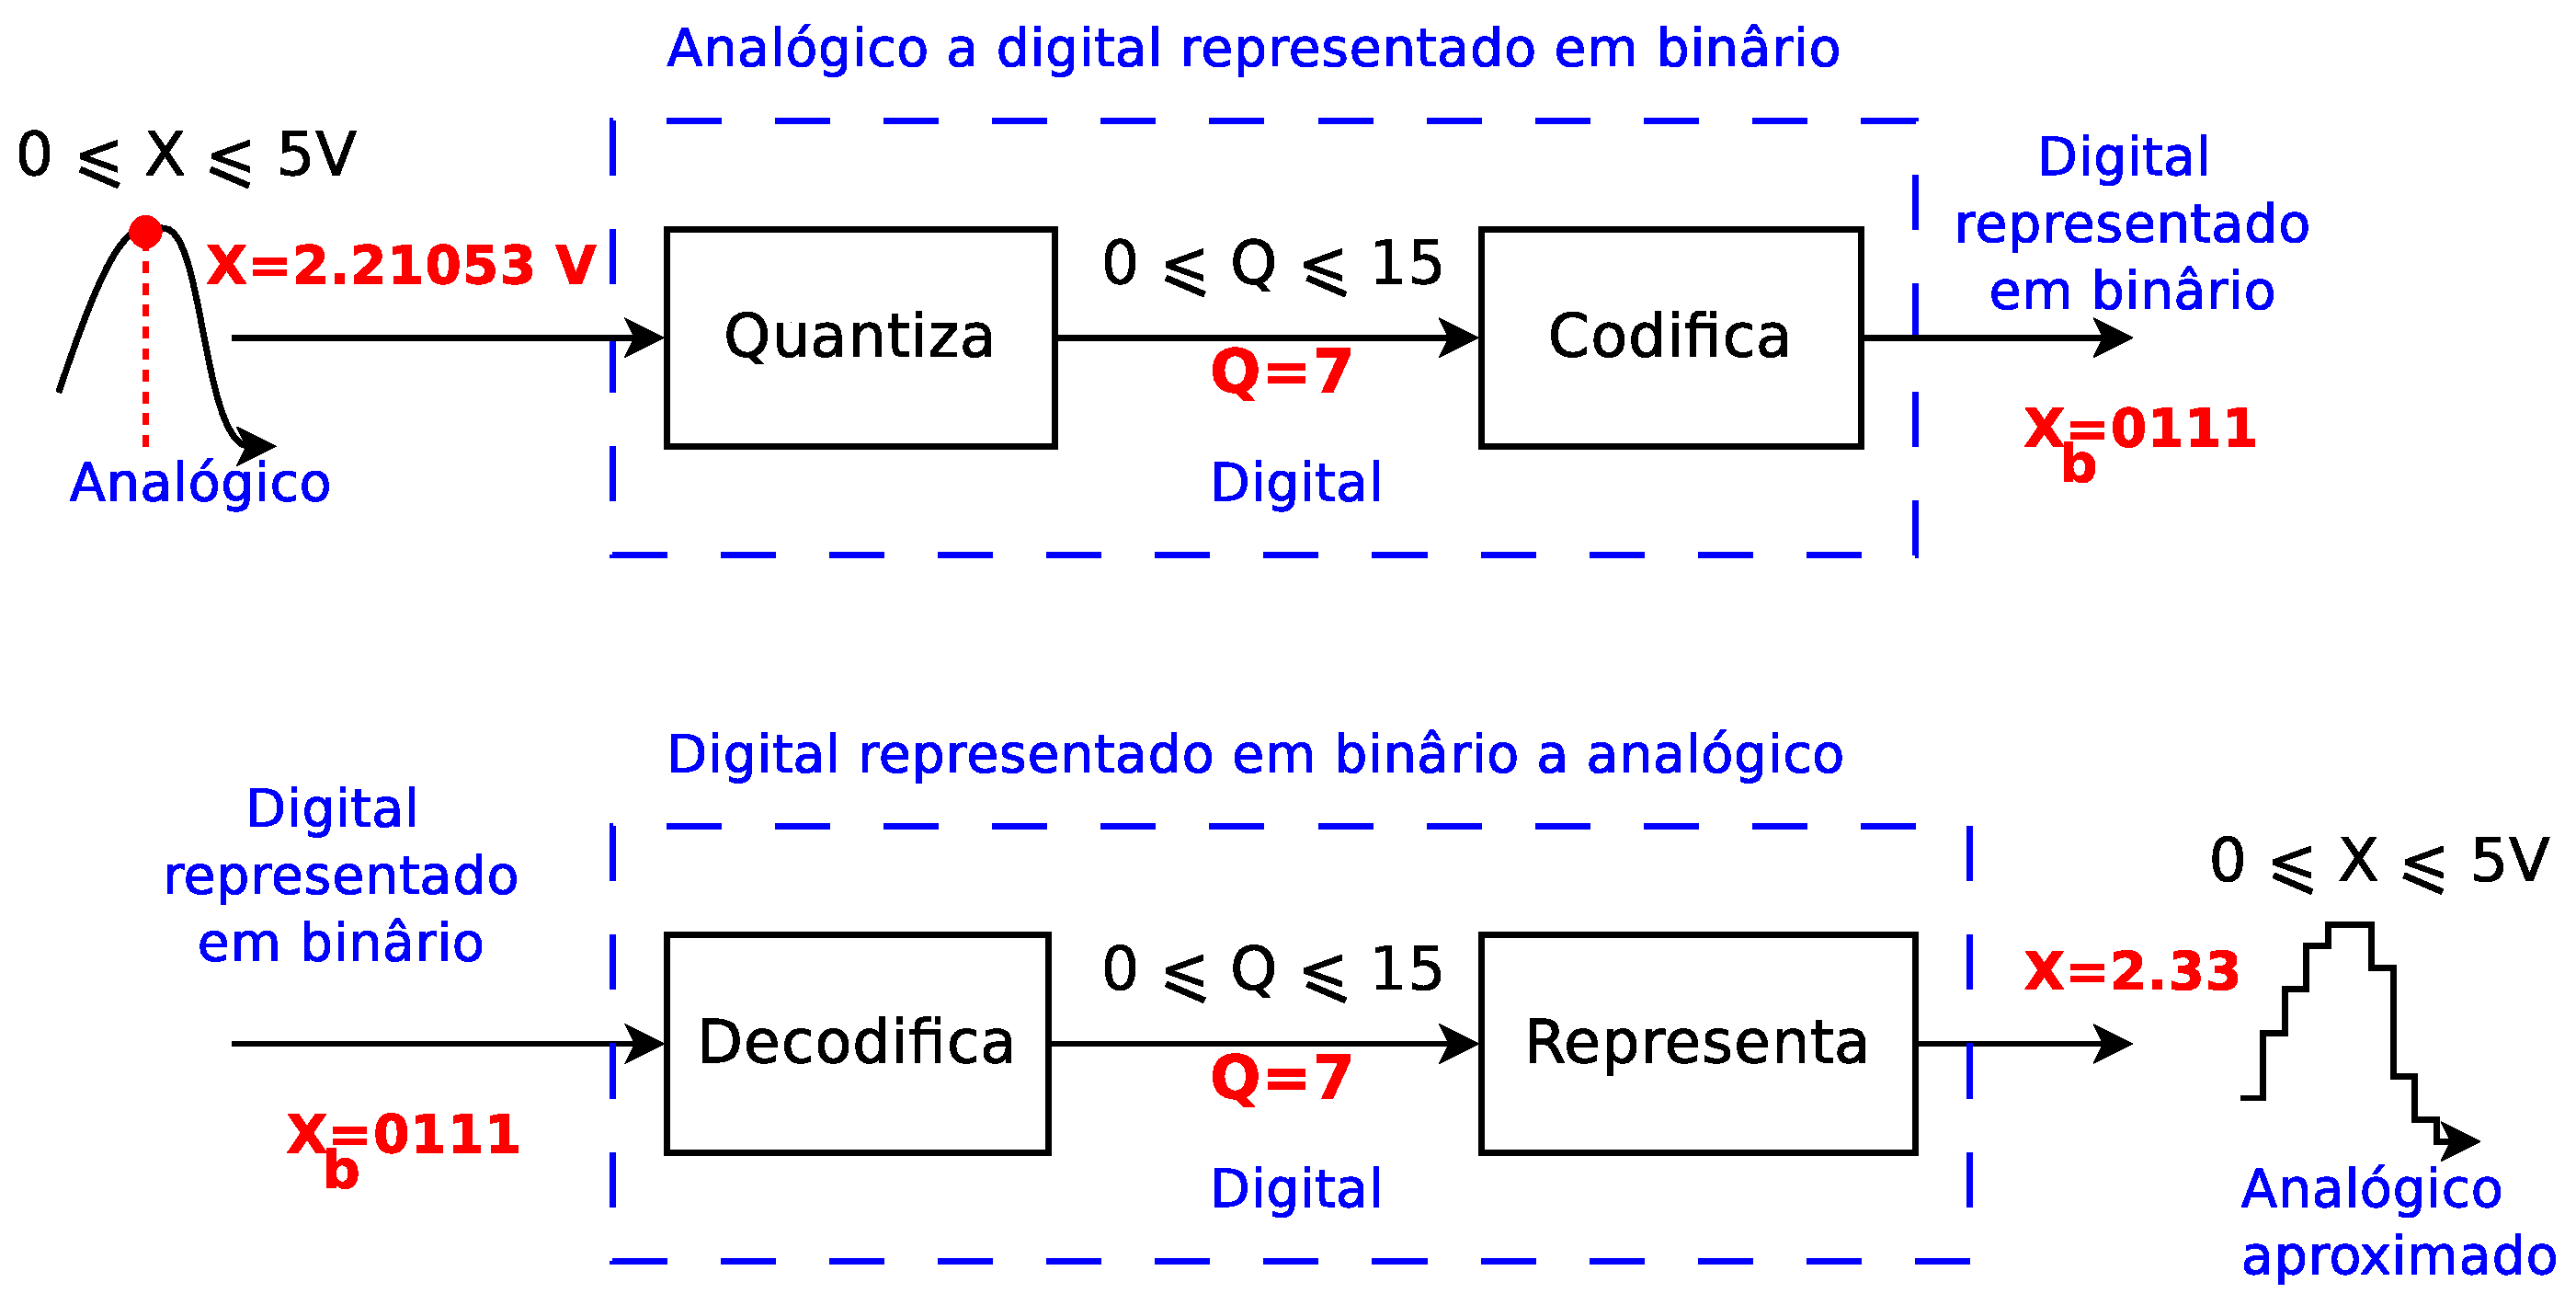
\includegraphics[width=1.0\textwidth]{images/Grafica0.eps}
\end{center} 
\end{frame}

%%%%%%%%%%%%%%%%%%%%%%%%%%%%%%%%%%%%%%%%%%%%%%%%%%%%%%%%%%%%%%%%%%%%%%%%%%%%%%%%
\begin{frame}{Conversão entre digital e analógico }
\begin{center}
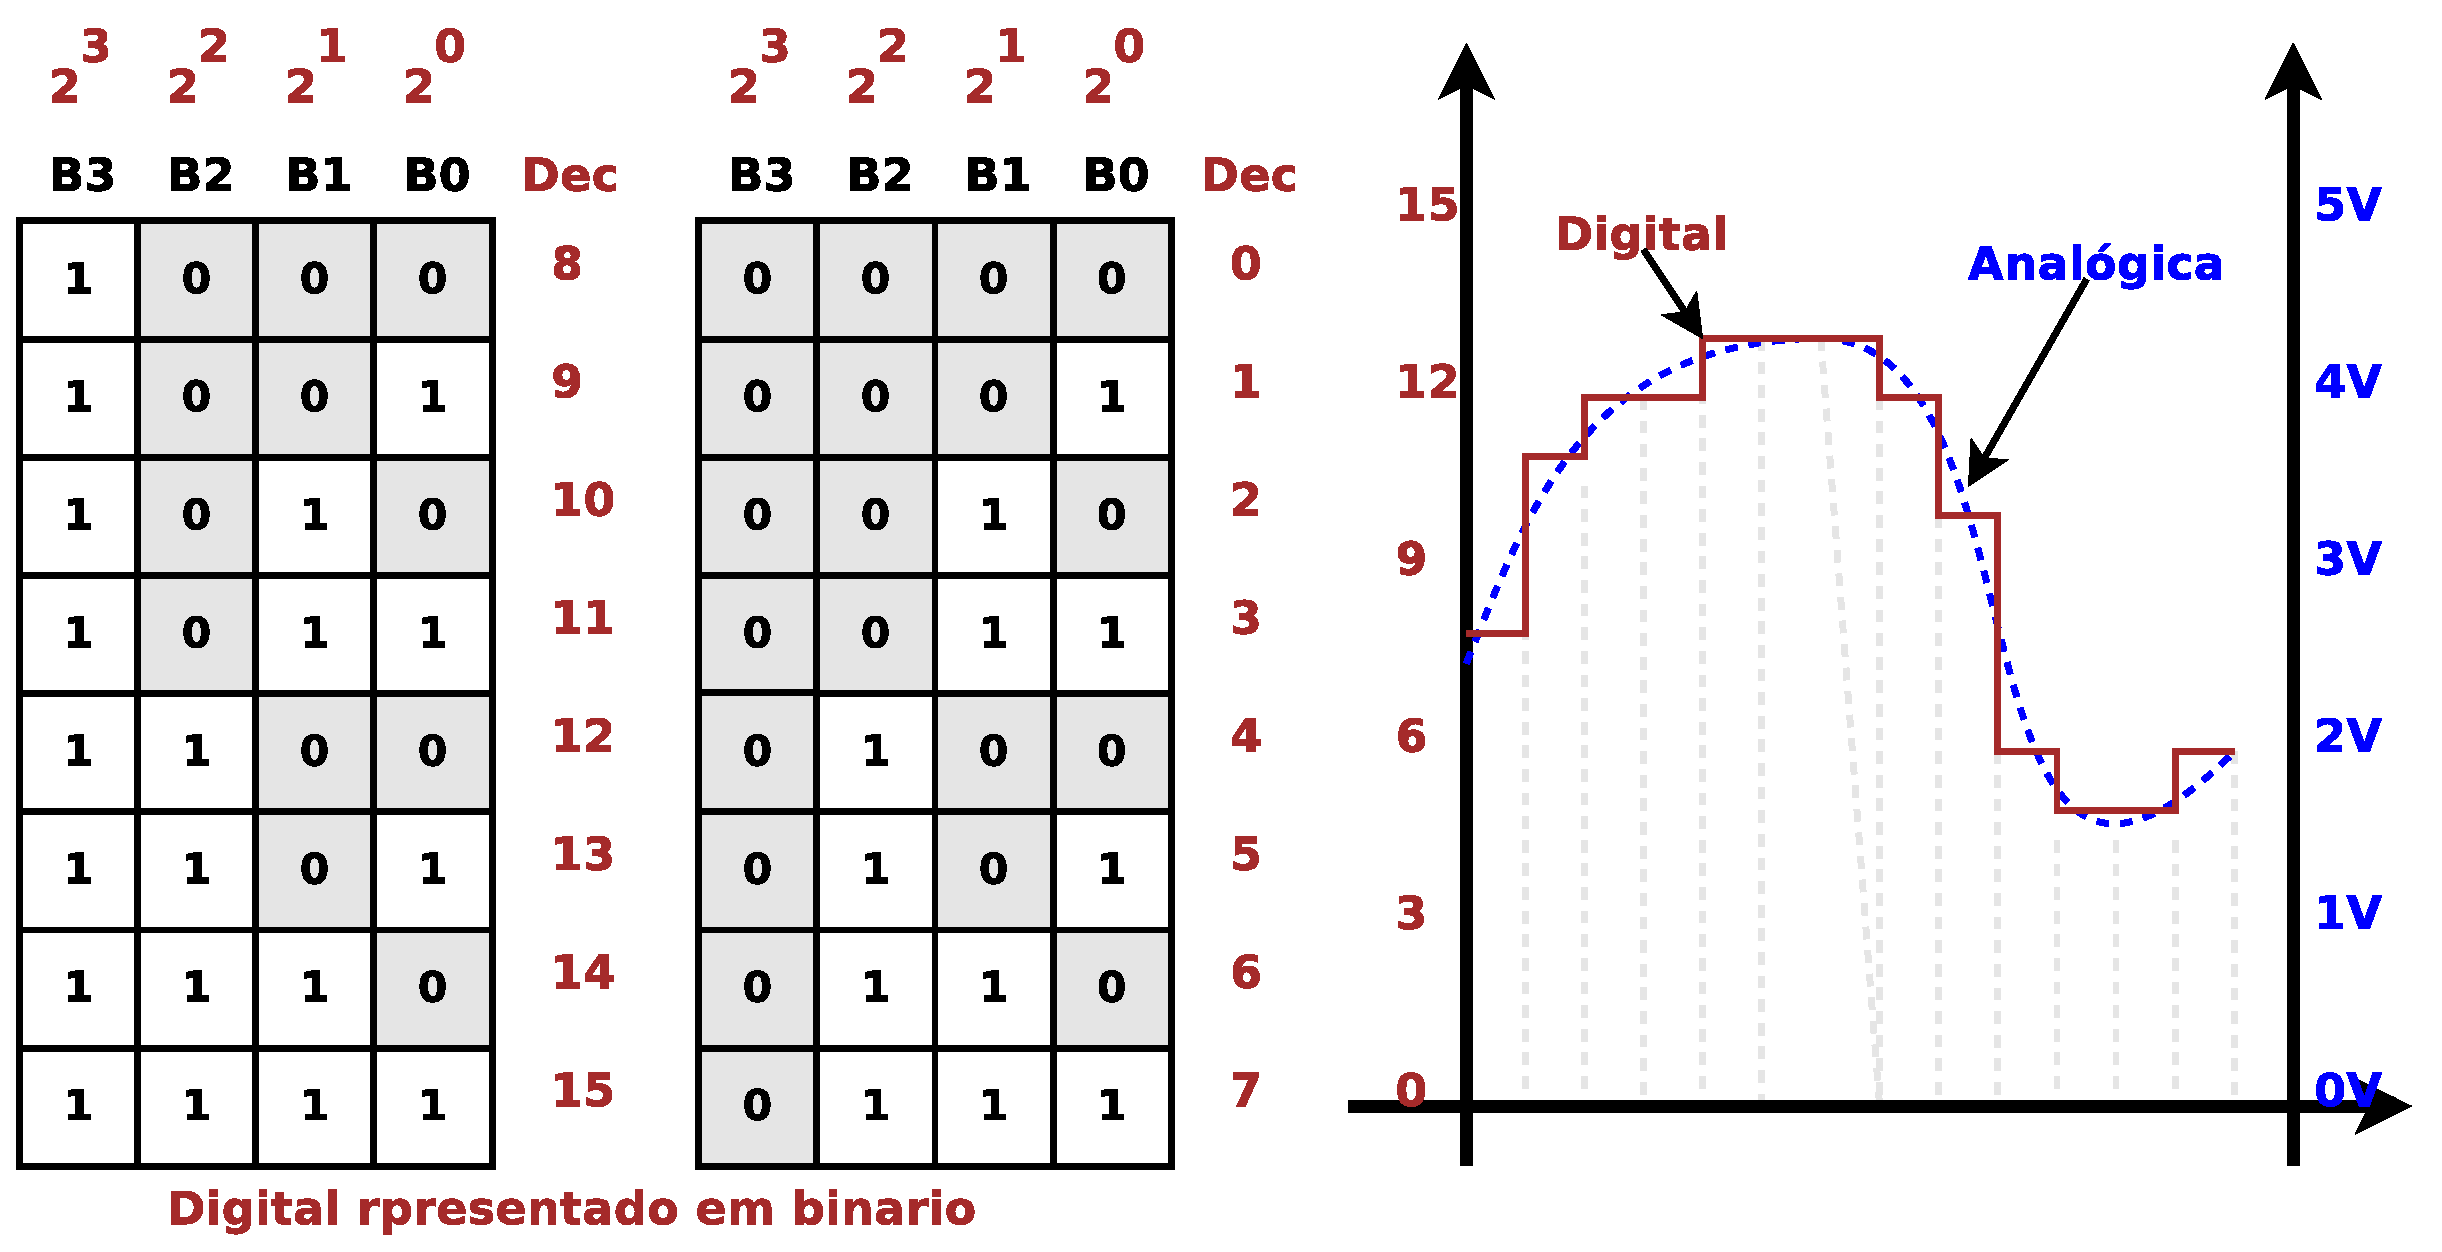
\includegraphics[width=1.0\textwidth]{images/Grafica1.eps}
\end{center} 
\end{frame}

%%%%%%%%%%%%%%%%%%%%%%%%%%%%%%%%%%%%%%%%%%%%%%%%%%%%%%%%%%%%%%%%%%%%%%%%%%%%%%%%
\begin{frame}{Conversão entre digital e analógico }
\begin{description}
 \item[Resolução porcentual:] $r=\frac{1}{2^n-1}100\%$. Exemplo: se $n=4$ a resolução
 é de 6.7\% do máximo voltagem de saída.Exemplo: se $n=12$ a resolução
 é de 0.024414\% do máximo voltagem de saída.
 \item[Exatidão:]  Máxima desviação do seu valor esperado. se expressa como porcentagem
 da saída máxima. Exemplo: Exatidão de $\pm 0.1\%$ tendo $5V$ de saída máxima, da
 um error de $5mV$
 \item[Linealidade:] Relação lineal entre o sinal digital ($S_d$) e a sinal analógica ($S_a$). É dizer
 sua relação está dada por $S_a=K_1 S_d + K_2$
\item[Tempo de resposta:] Tempo entre que se recebe um dado e este é interpretado.
\end{description}  
\end{frame}

%%%%%%%%%%%%%%%%%%%%%%%%%%%%%%%%%%%%%%%%%%%%%%%%%%%%%%%%%%%%%%%%%%%%%%%%%%%%%%%%
%%%%%%%%%%%%%%%%%%%%%%%%%%%%%%%%%%%%%%%%%%%%%%%%%%%%%%%%%%%%%%%%%%%%%%%%%%%%%%%%
%%%%%%%%%%%%%%%%%%%%%%%%%%%%%%%%%%%%%%%%%%%%%%%%%%%%%%%%%%%%%%%%%%%%%%%%%%%%%%%%
\section{Conversão DA}
%%%%%%%%%%%%%%%%%%%%%%%%%%%%%%%%%%%%%%%%%%%%%%%%%%%%%%%%%%%%%%%%%%%%%%%%%%%%%%%%
\begin{frame}{Conversão digital-analógico}
\begin{center}
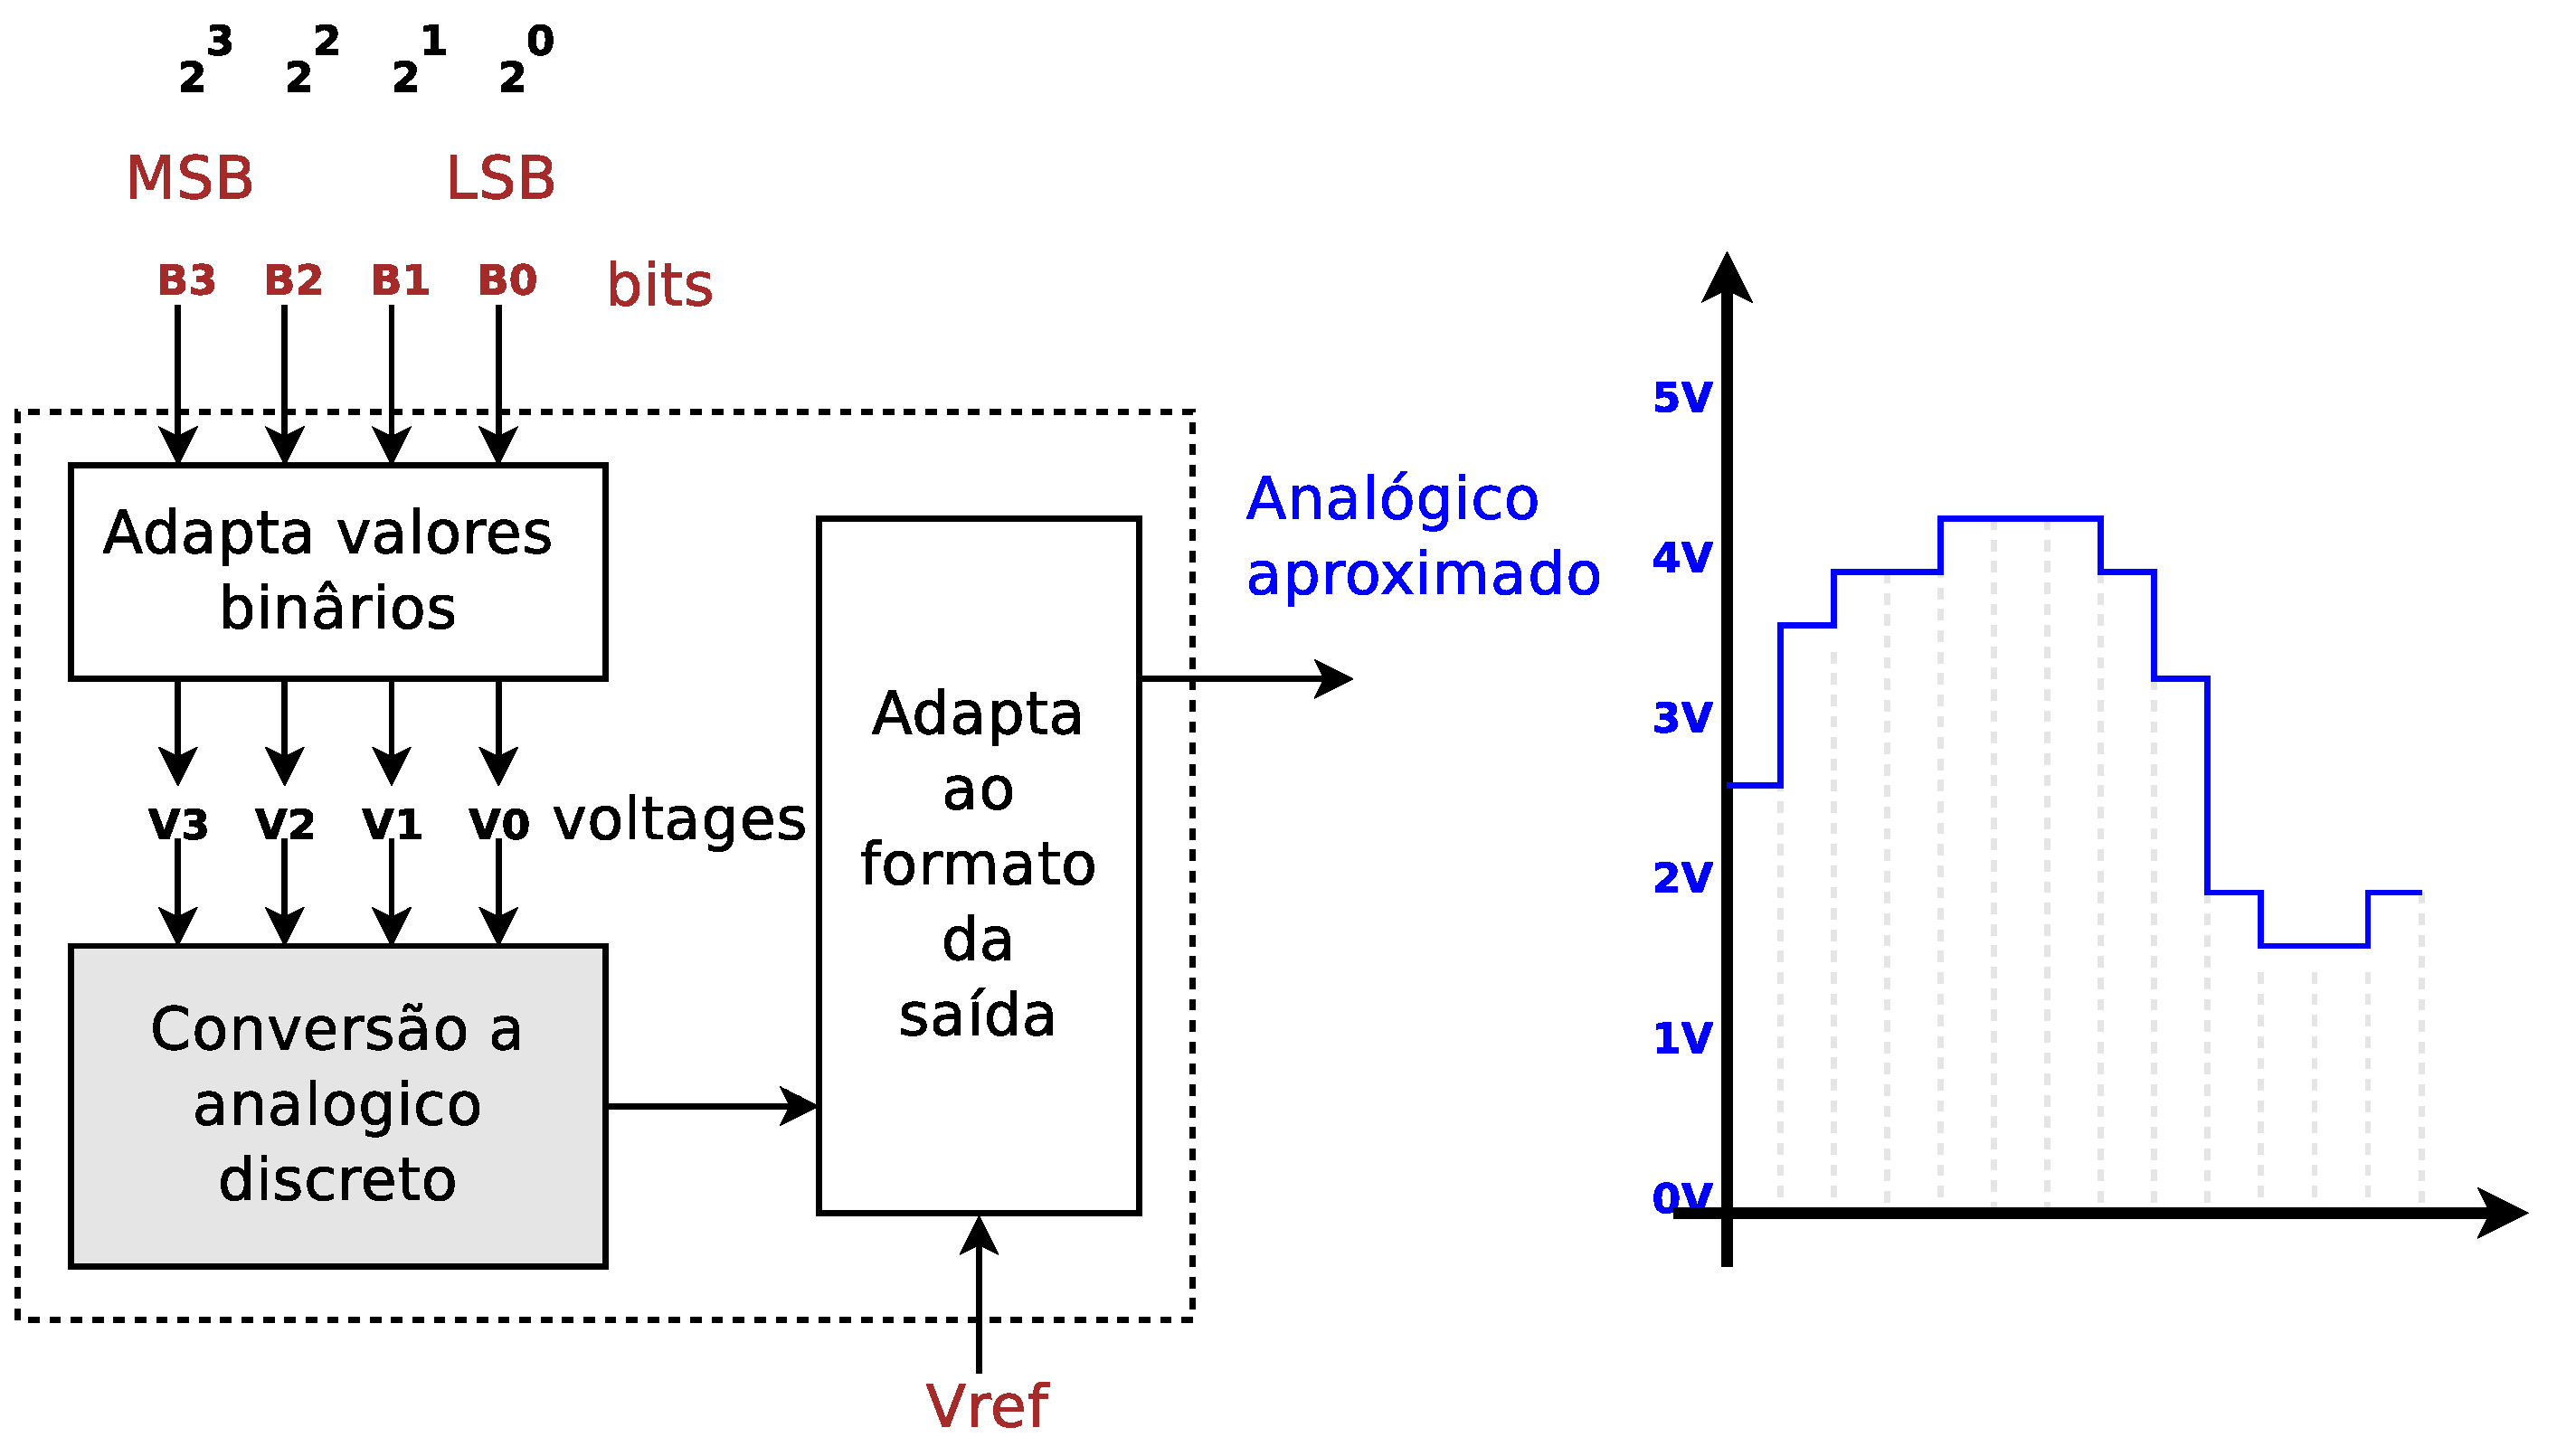
\includegraphics[width=1.0\textwidth]{images/DA.eps}
\end{center} 
\end{frame}
%%%%%%%%%%%%%%%%%%%%%%%%%%%%%%%%%%%%%%%%%%%%%%%%%%%%%%%%%%%%%%%%%%%%%%%%%%%%%%%%
%http://endigital.orgfree.com/sequencial/conversorDA.htm
\begin{frame}{Conversão digital-analógico de entrada ponderada}
\begin{minipage}[c]{0.5\textwidth}
\begin{center}
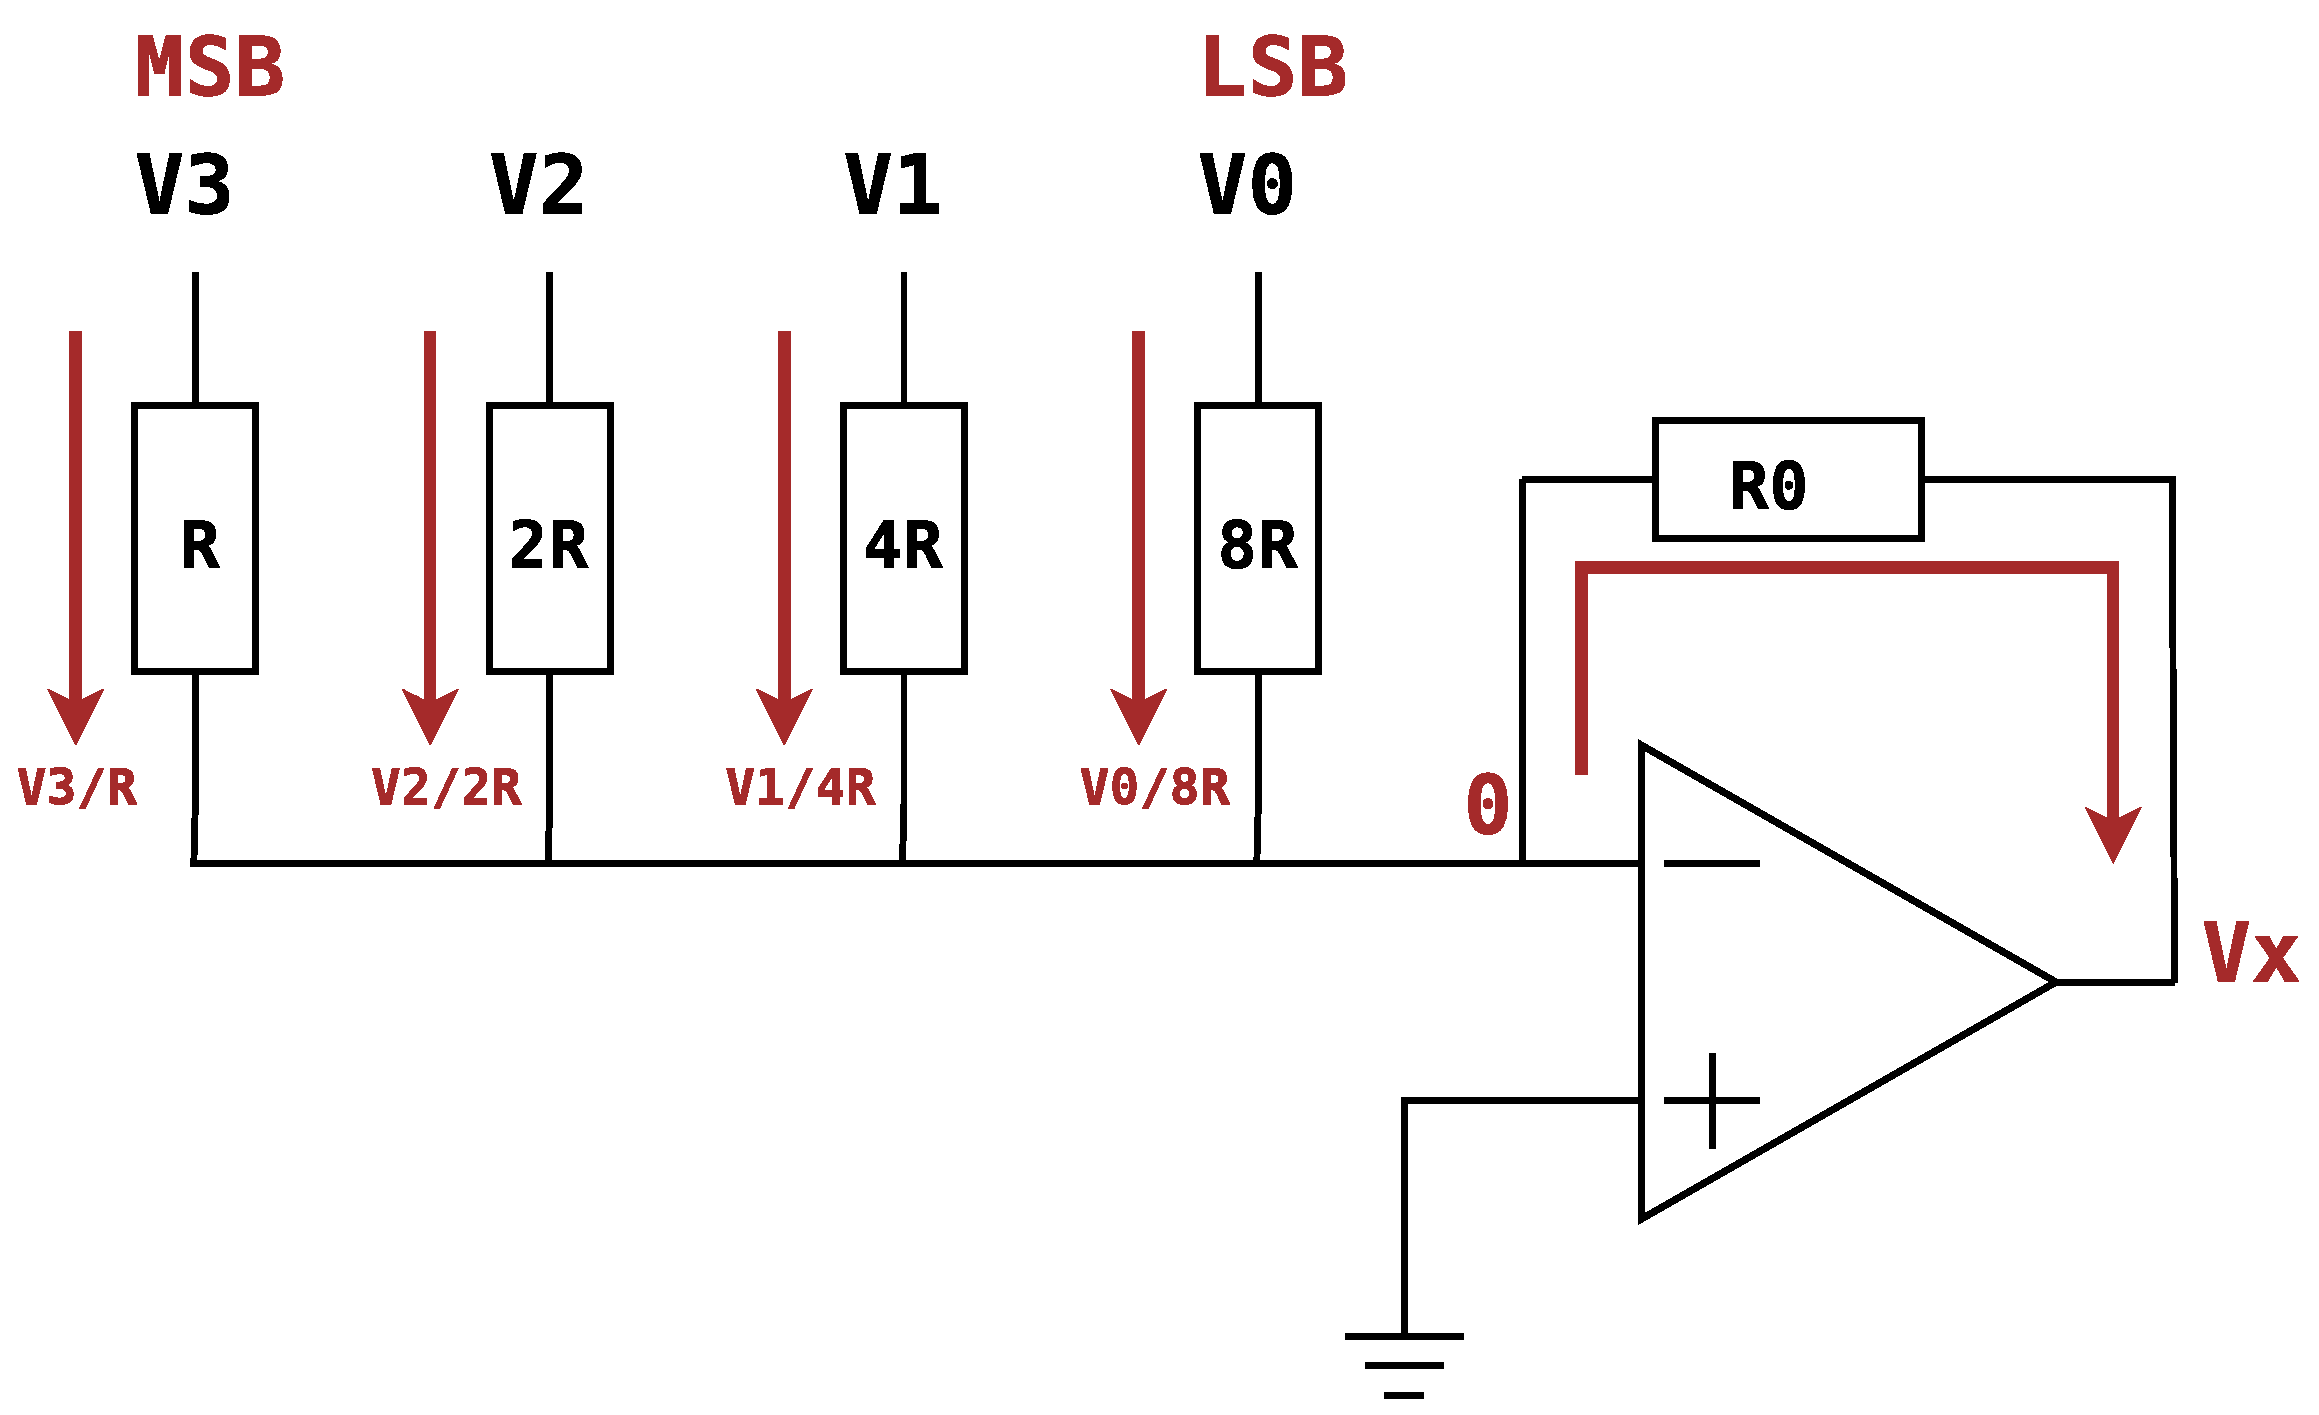
\includegraphics[width=0.9\textwidth]{images/ADmodelo1.eps}
\end{center} 
\end{minipage}%
\begin{minipage}[c]{0.5\textwidth}
\begin{block}{Soma das correntes no nó}
\small
\begin{equation*}
 V_x=-R_0\frac{(  V_0 + 2 V_1 + 4 V_2 + 8 V_3 )}{8R}
\end{equation*}
\normalsize
\end{block} 
\begin{block}{Desvantagens}
\begin{itemize}
 \item Precisa muitos tipos diferentes de resistências.
  \item Pode trazer erros pela tolerância porcentual das resistências.
\end{itemize}
\end{block} 
\end{minipage}
\end{frame}

%%%%%%%%%%%%%%%%%%%%%%%%%%%%%%%%%%%%%%%%%%%%%%%%%%%%%%%%%%%%%%%%%%%%%%%%%%%%%%%%%
%http://endigital.orgfree.com/sequencial/conversorDA.htm
%http://hyperphysics.phy-astr.gsu.edu/hbasees/electronic/dac.html
%http://es.slideshare.net/ruben_loredo/interfazamiento-de-sistemas-digital-analogo-presentation
%https://www.youtube.com/watch?v=FNLnyGZOS10
\begin{frame}{Conversão digital-analogico com rede tipo R-2R \cite{boylestad2004dispositivos}}
\begin{center}
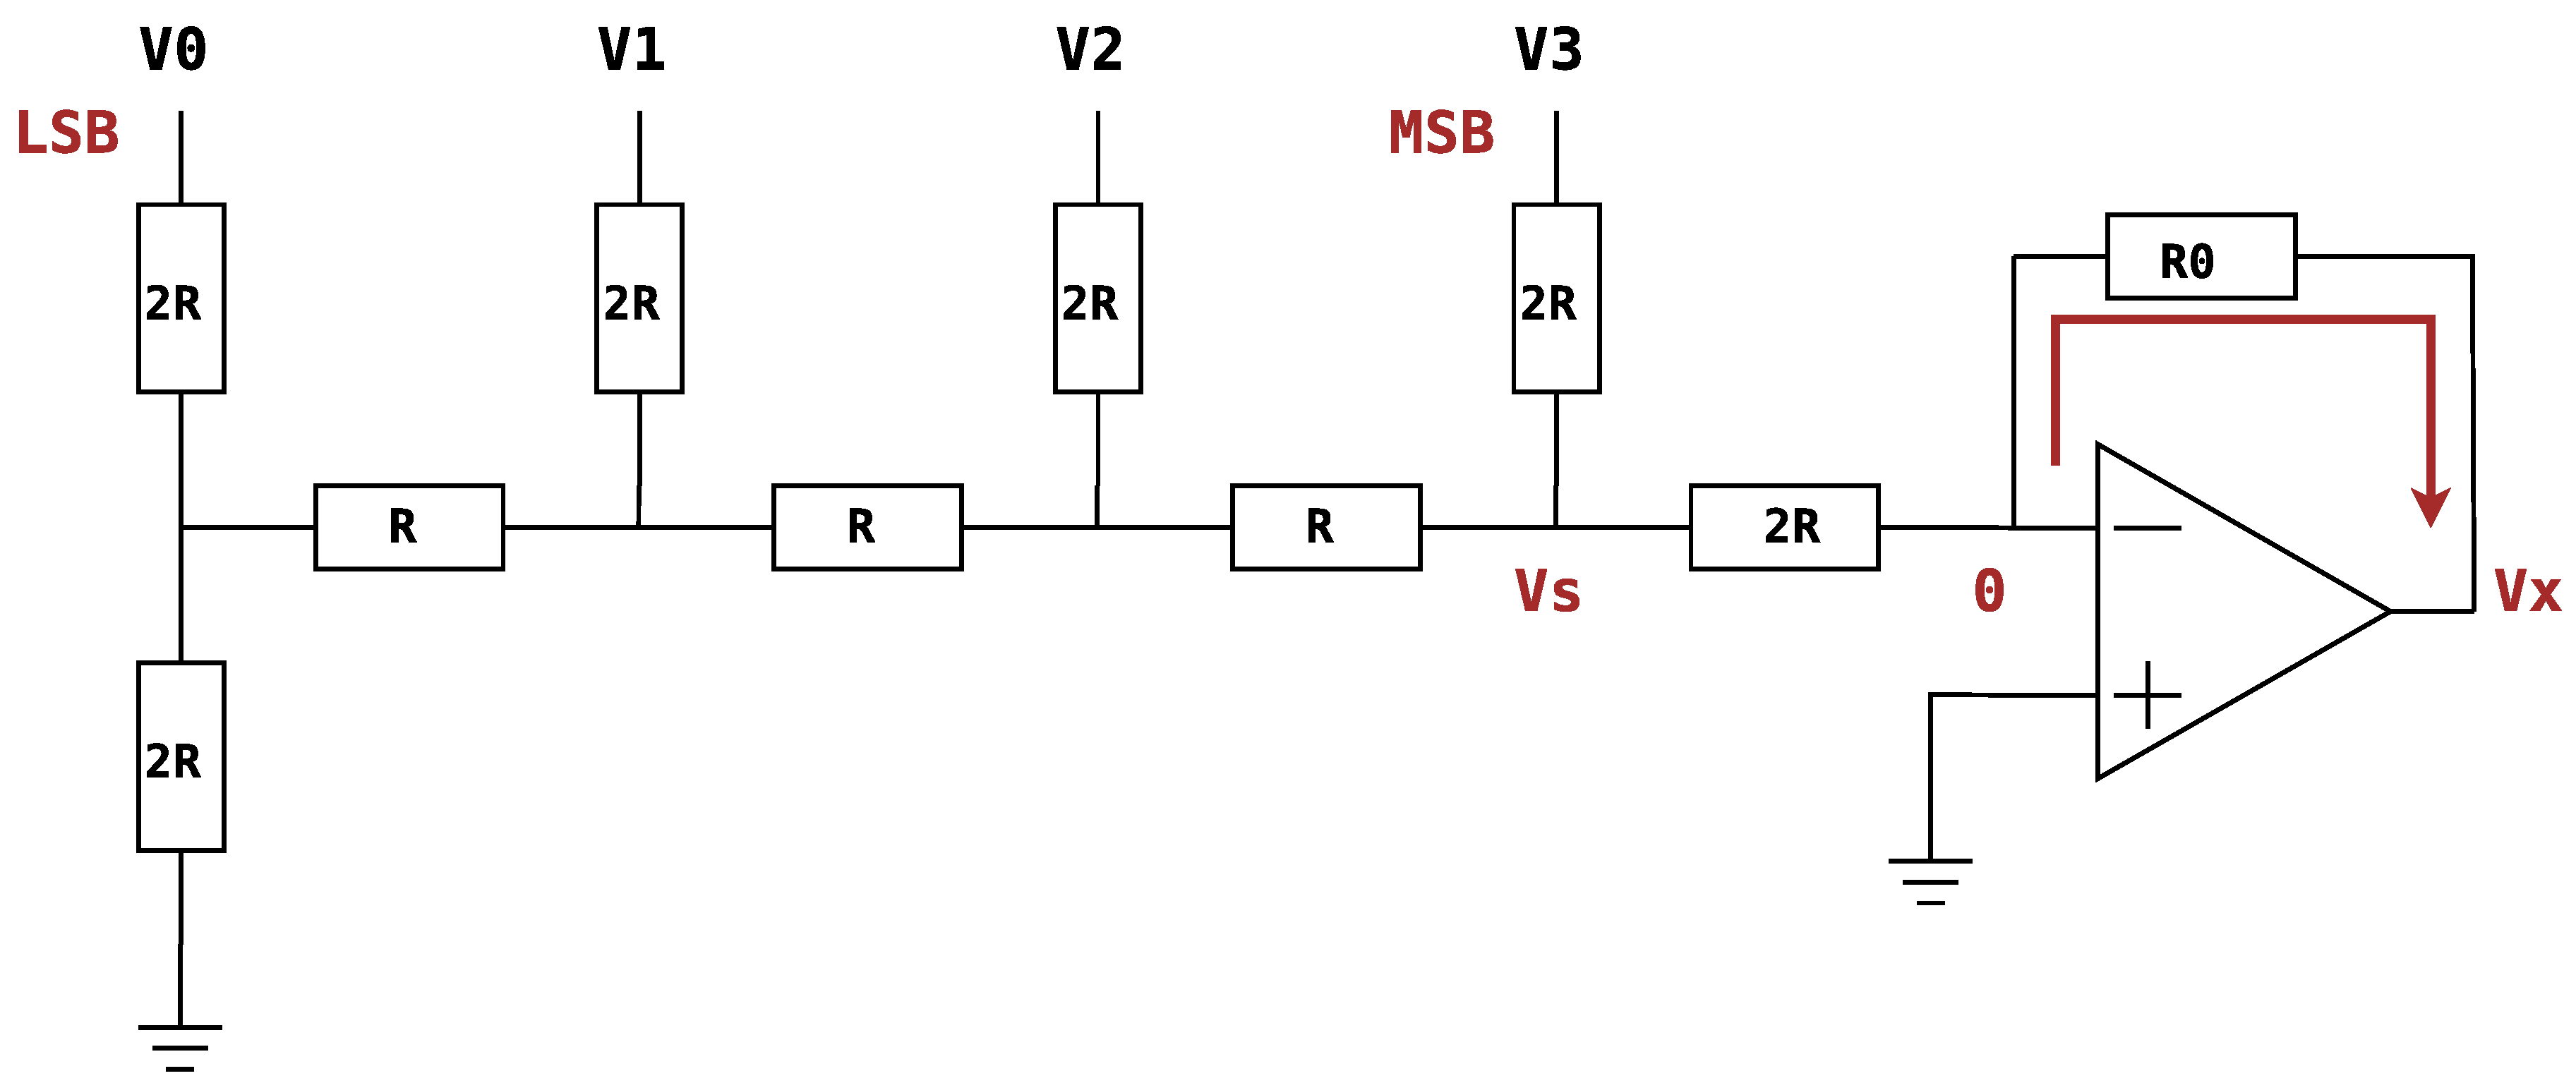
\includegraphics[width=0.7\textwidth]{images/ADmodelo2.eps}
\end{center} 
\begin{block}{Teorema de superposição}
\small
\begin{equation*}
 V_x=-\frac{R_0}{6R} \frac{(2^0V_0 + 2^1 V_1 + 2^2 V_2 + 2^3 V_3  )}{2^3}
\end{equation*}
\normalsize
\end{block} 
\end{frame}
%%%%%%%%%%%%
\begin{comment}
\begin{frame}{Conversão digital-analogico com rede tipo R-2R}
\begin{center}
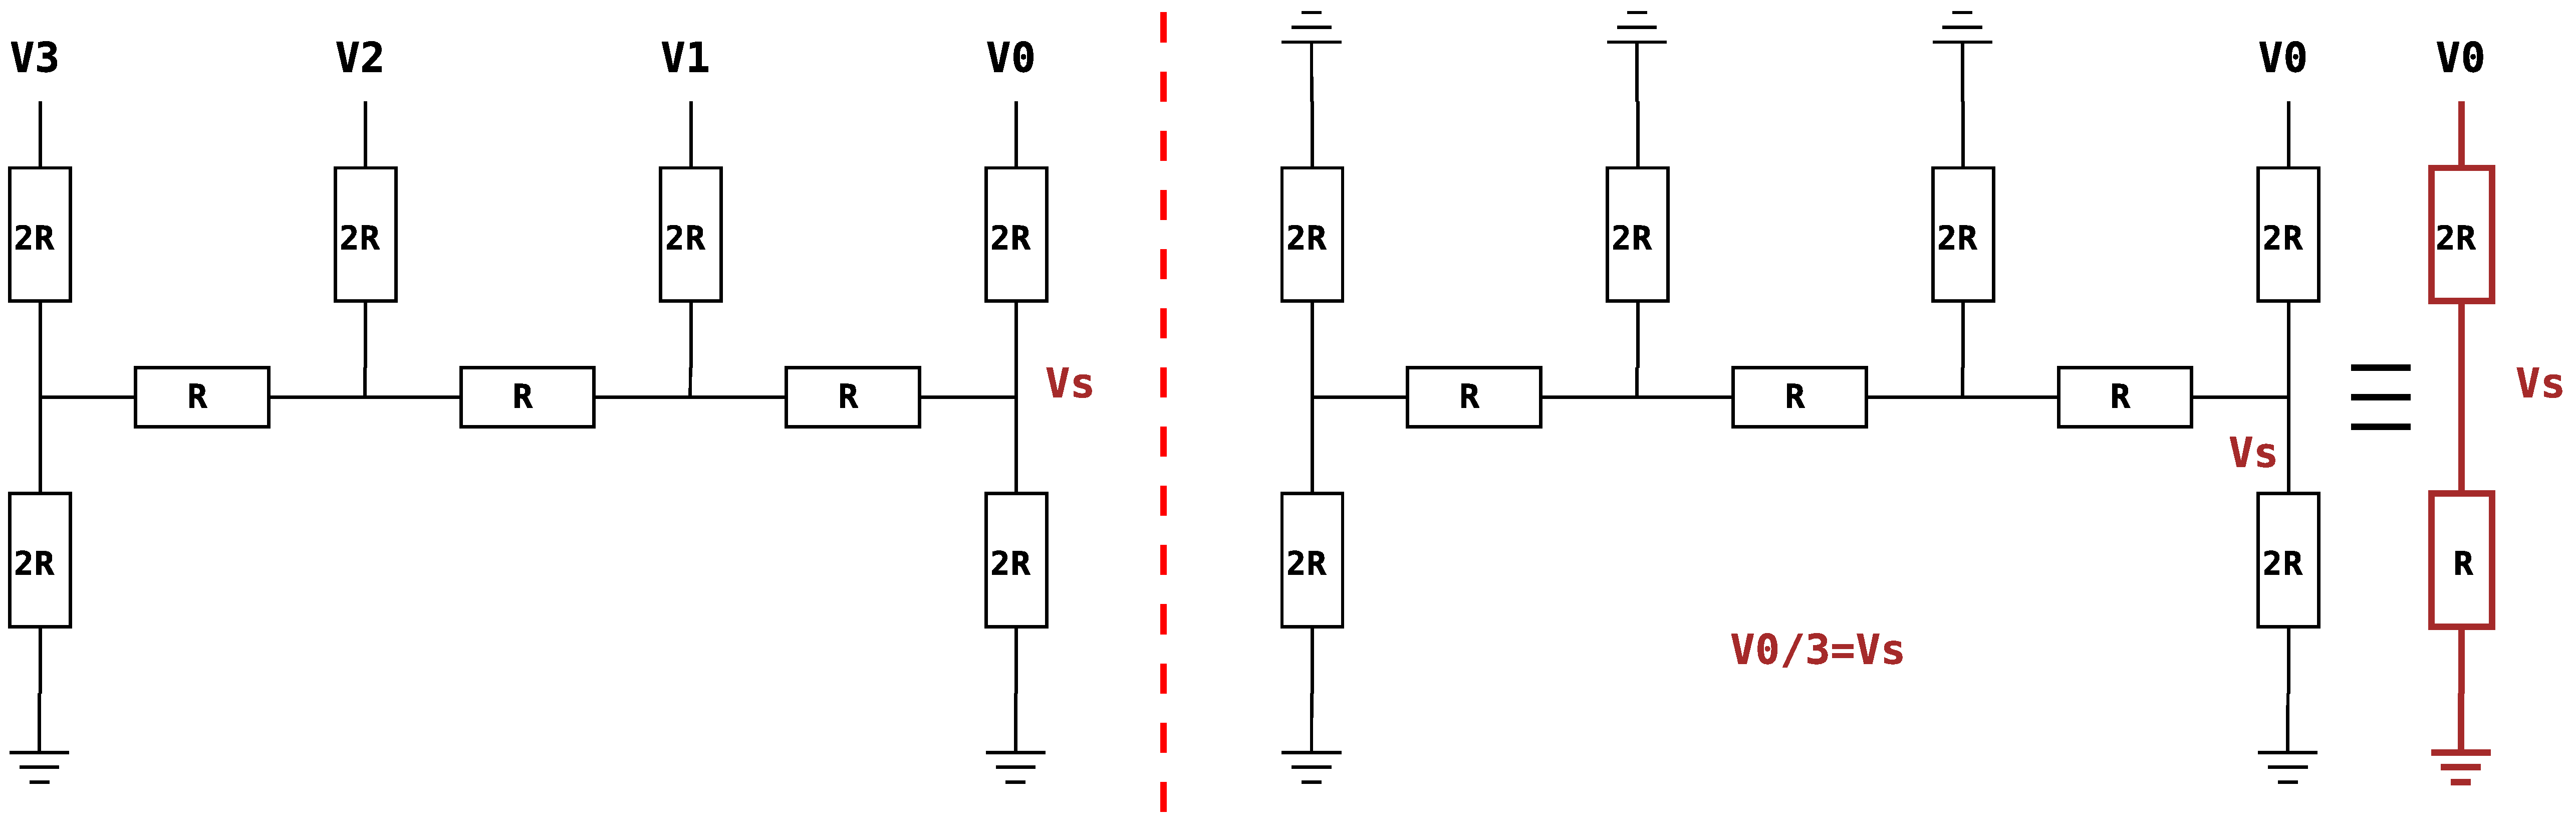
\includegraphics[width=1.0\textwidth]{images/Diagrama1.eps}
\end{center}
\end{frame}
\begin{frame}{Conversão digital-analogico com rede tipo R-2R}
\begin{center}
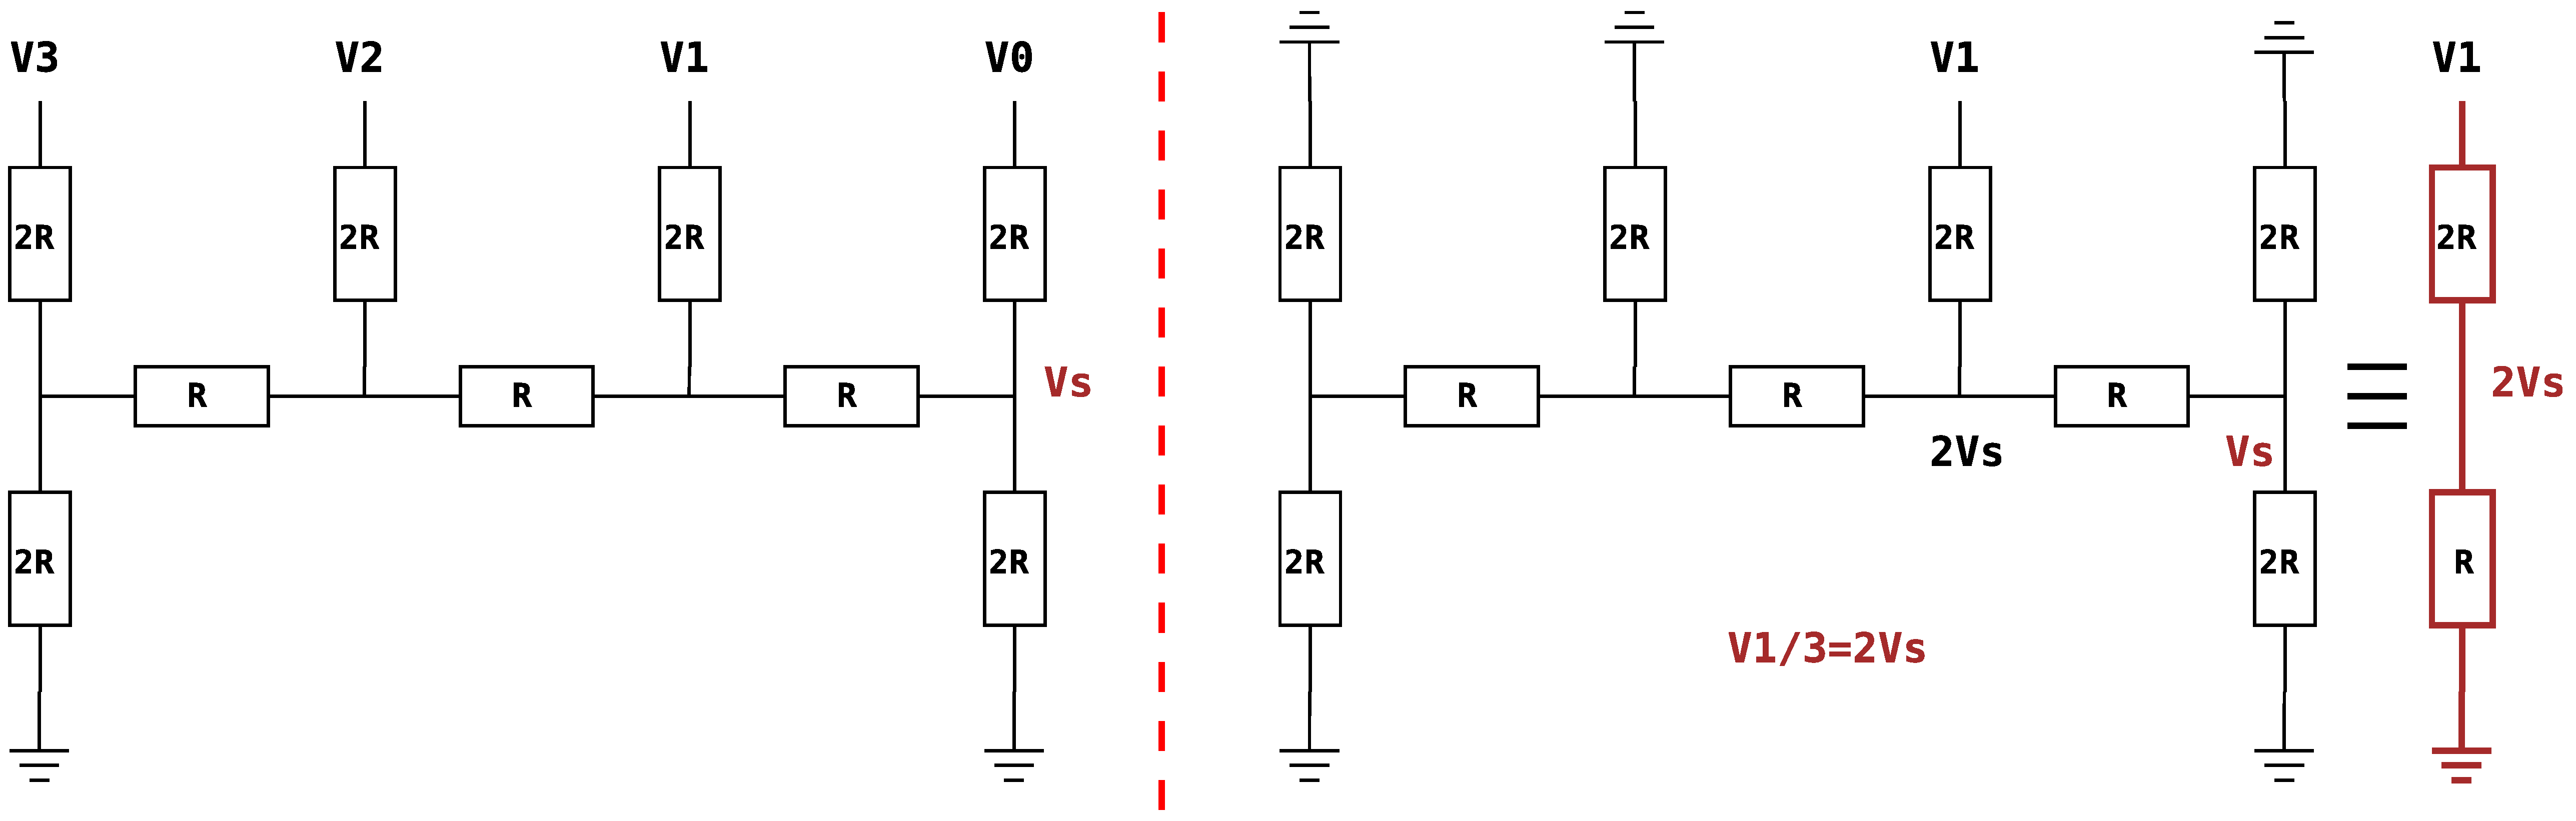
\includegraphics[width=1.0\textwidth]{images/Diagrama2.eps}
\end{center}
\end{frame}
\begin{frame}{Conversão digital-analogico com rede tipo R-2R}
\begin{center}
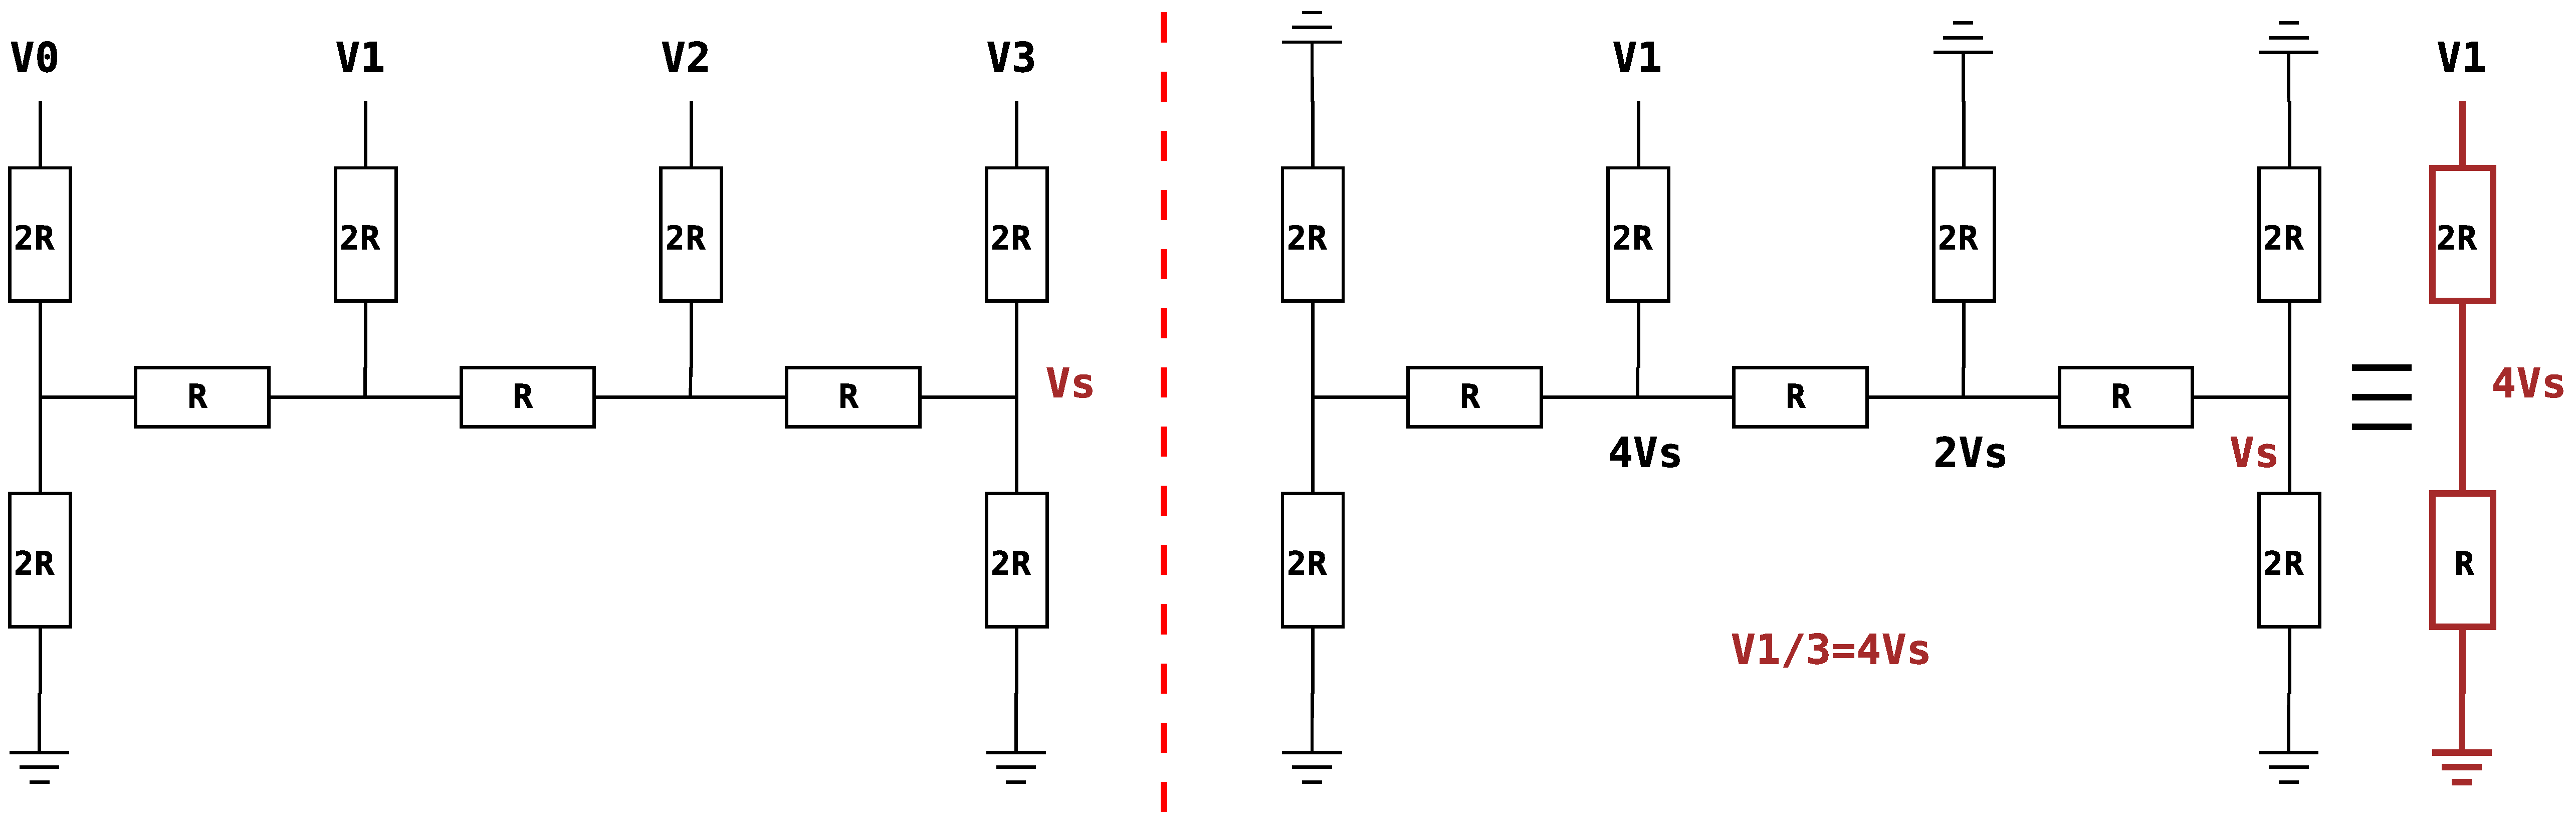
\includegraphics[width=1.0\textwidth]{images/Diagrama3.eps}
\end{center}
\end{frame}
\begin{frame}{Conversão digital-analogico com rede tipo R-2R}
\begin{center}
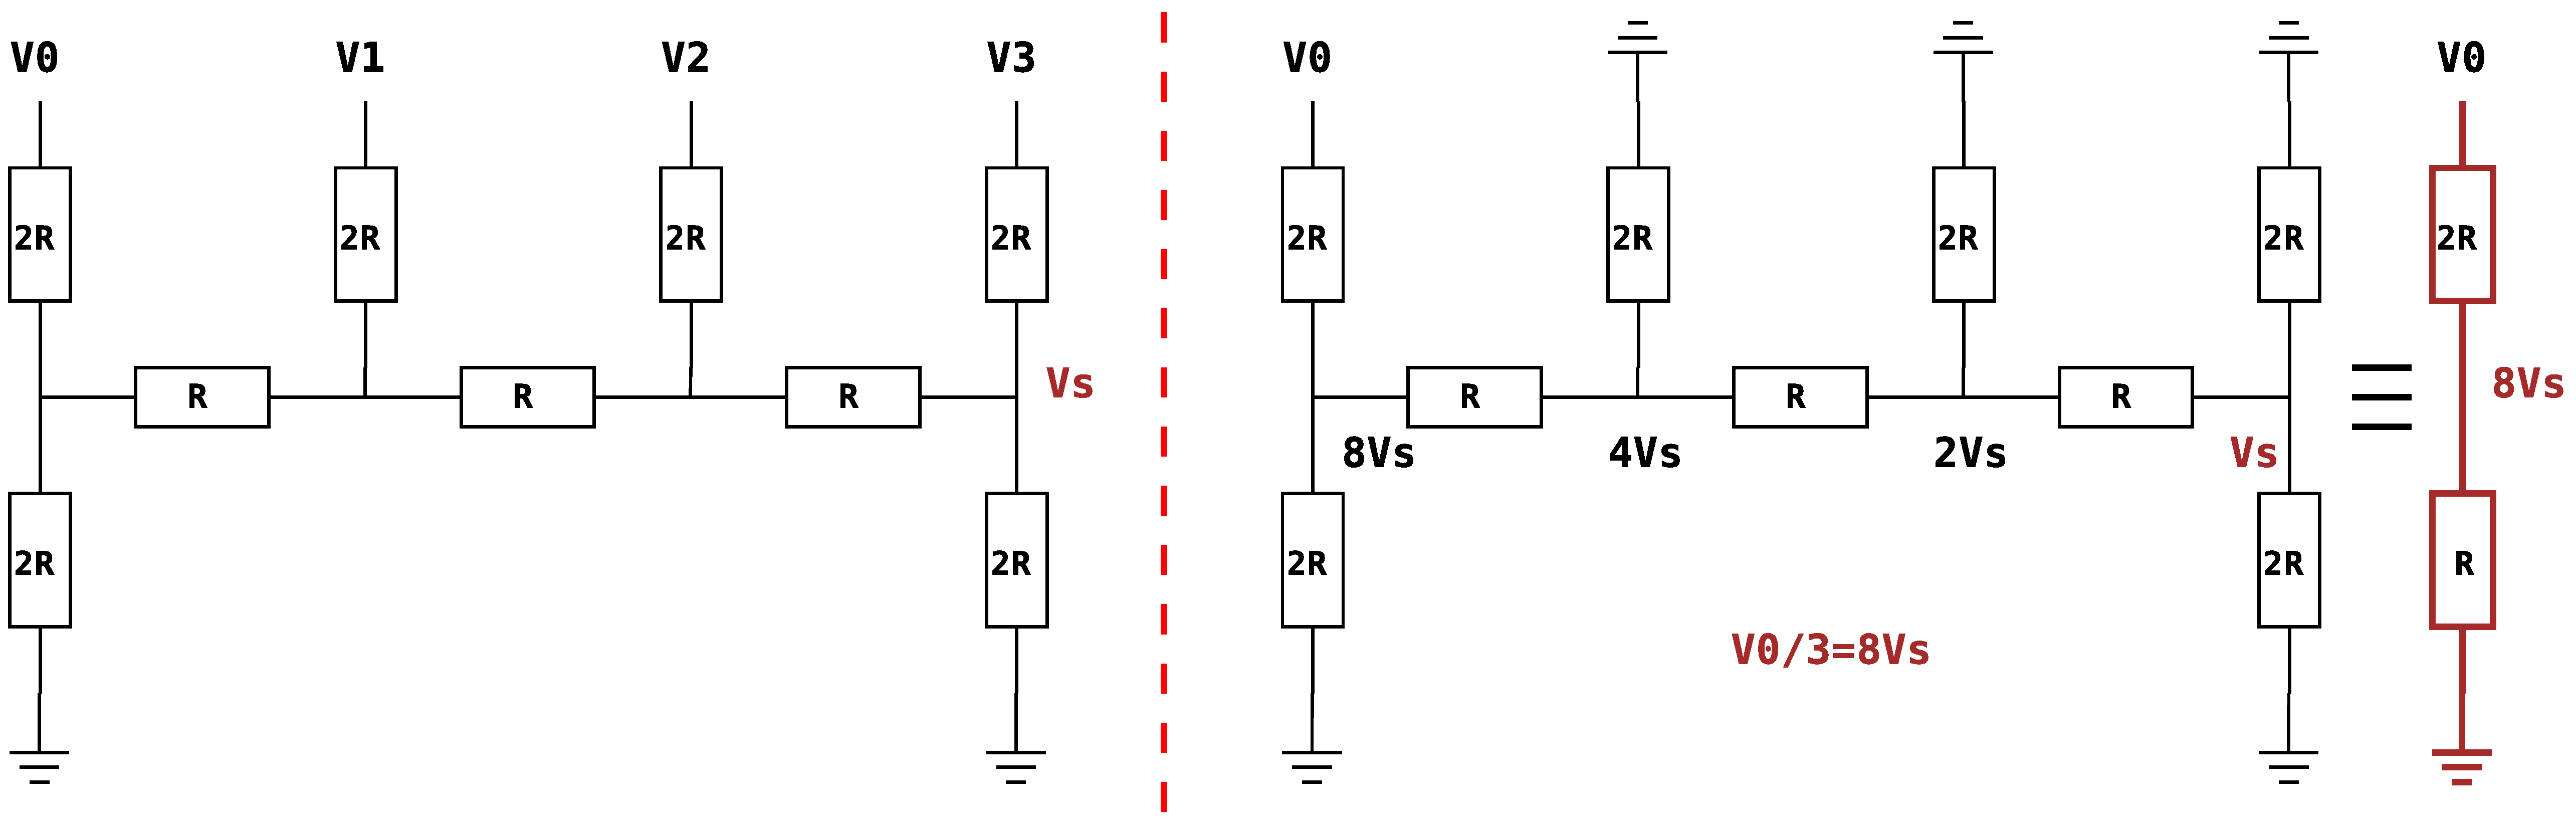
\includegraphics[width=1.0\textwidth]{images/Diagrama4.eps}
\end{center}
\end{frame}
\end{comment}
\begin{frame}{Conversão digital-analogico com rede tipo R-2R}
\begin{center}
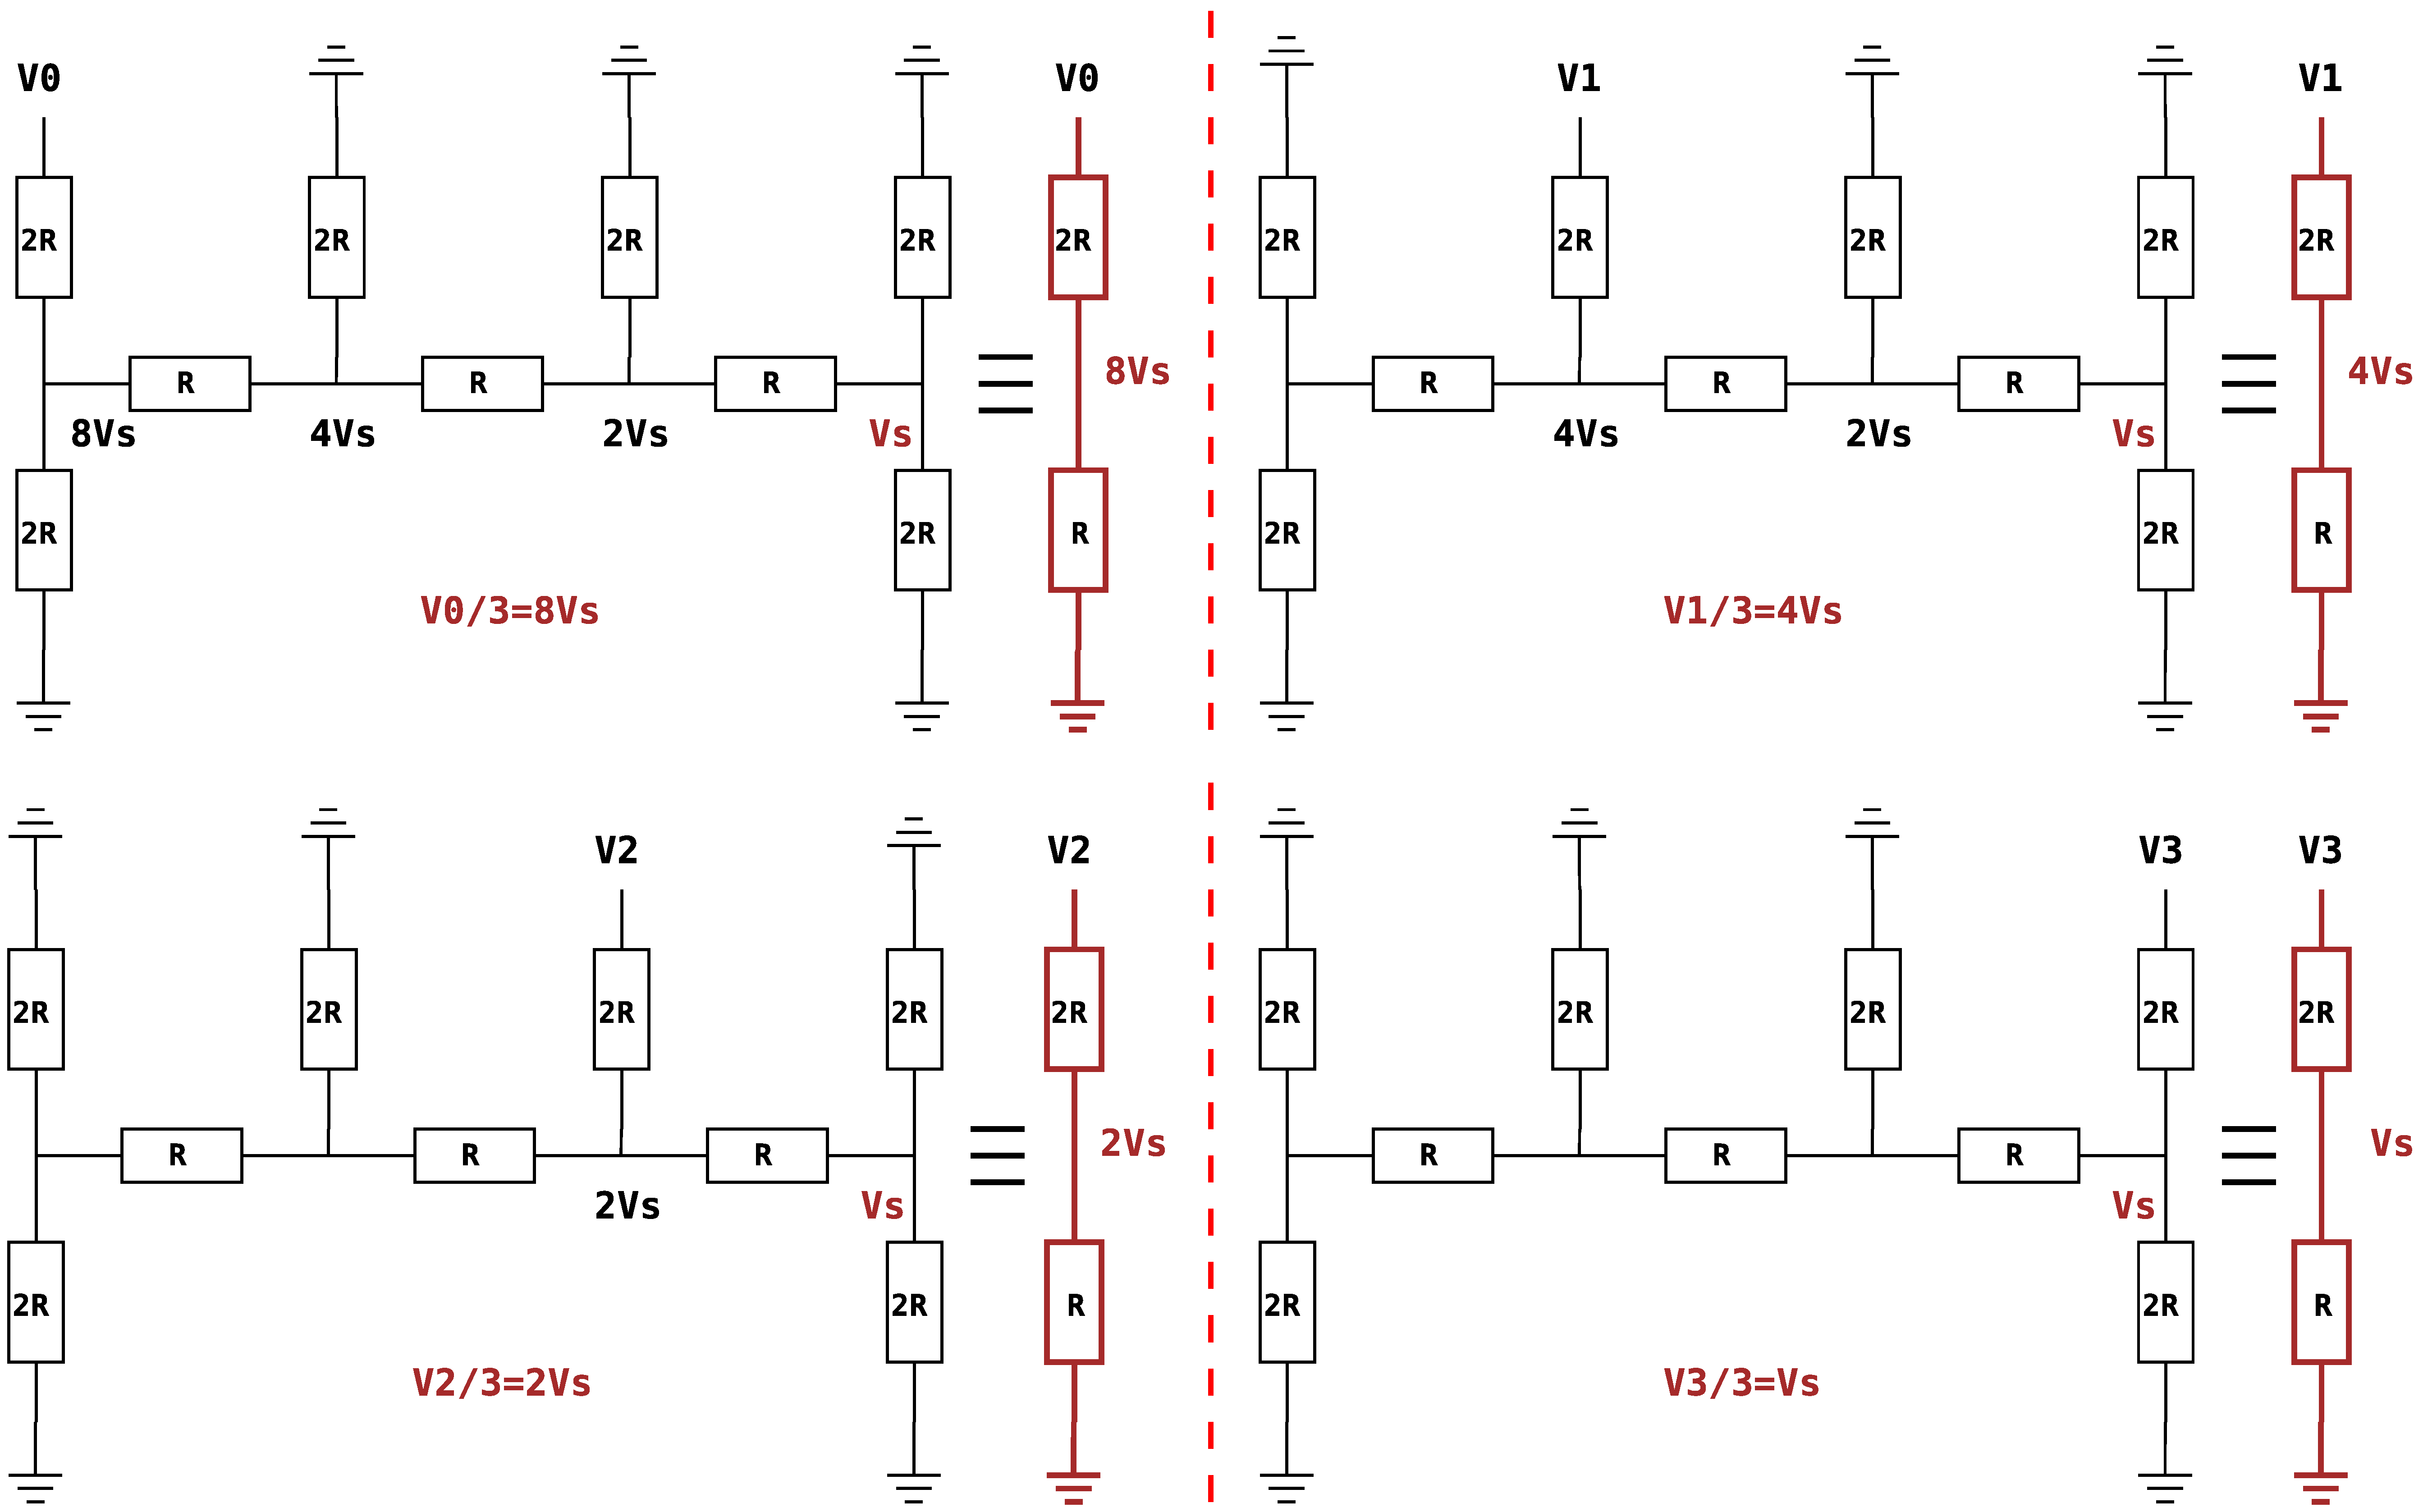
\includegraphics[width=1.0\textwidth]{images/DiagramaAll.eps}
\end{center}
\end{frame}
\begin{frame}{Conversão digital-analogico com rede tipo R-2R}
\begin{block}{Teorema de superposição}
\begin{equation*}
 V_s=\frac{1}{3} \frac{(2^0 V_0 + 2^1 V_1 + 2^2 V_2 + 2^3 V_3 )}{2^3}
\end{equation*}
\end{block} 
\begin{center}
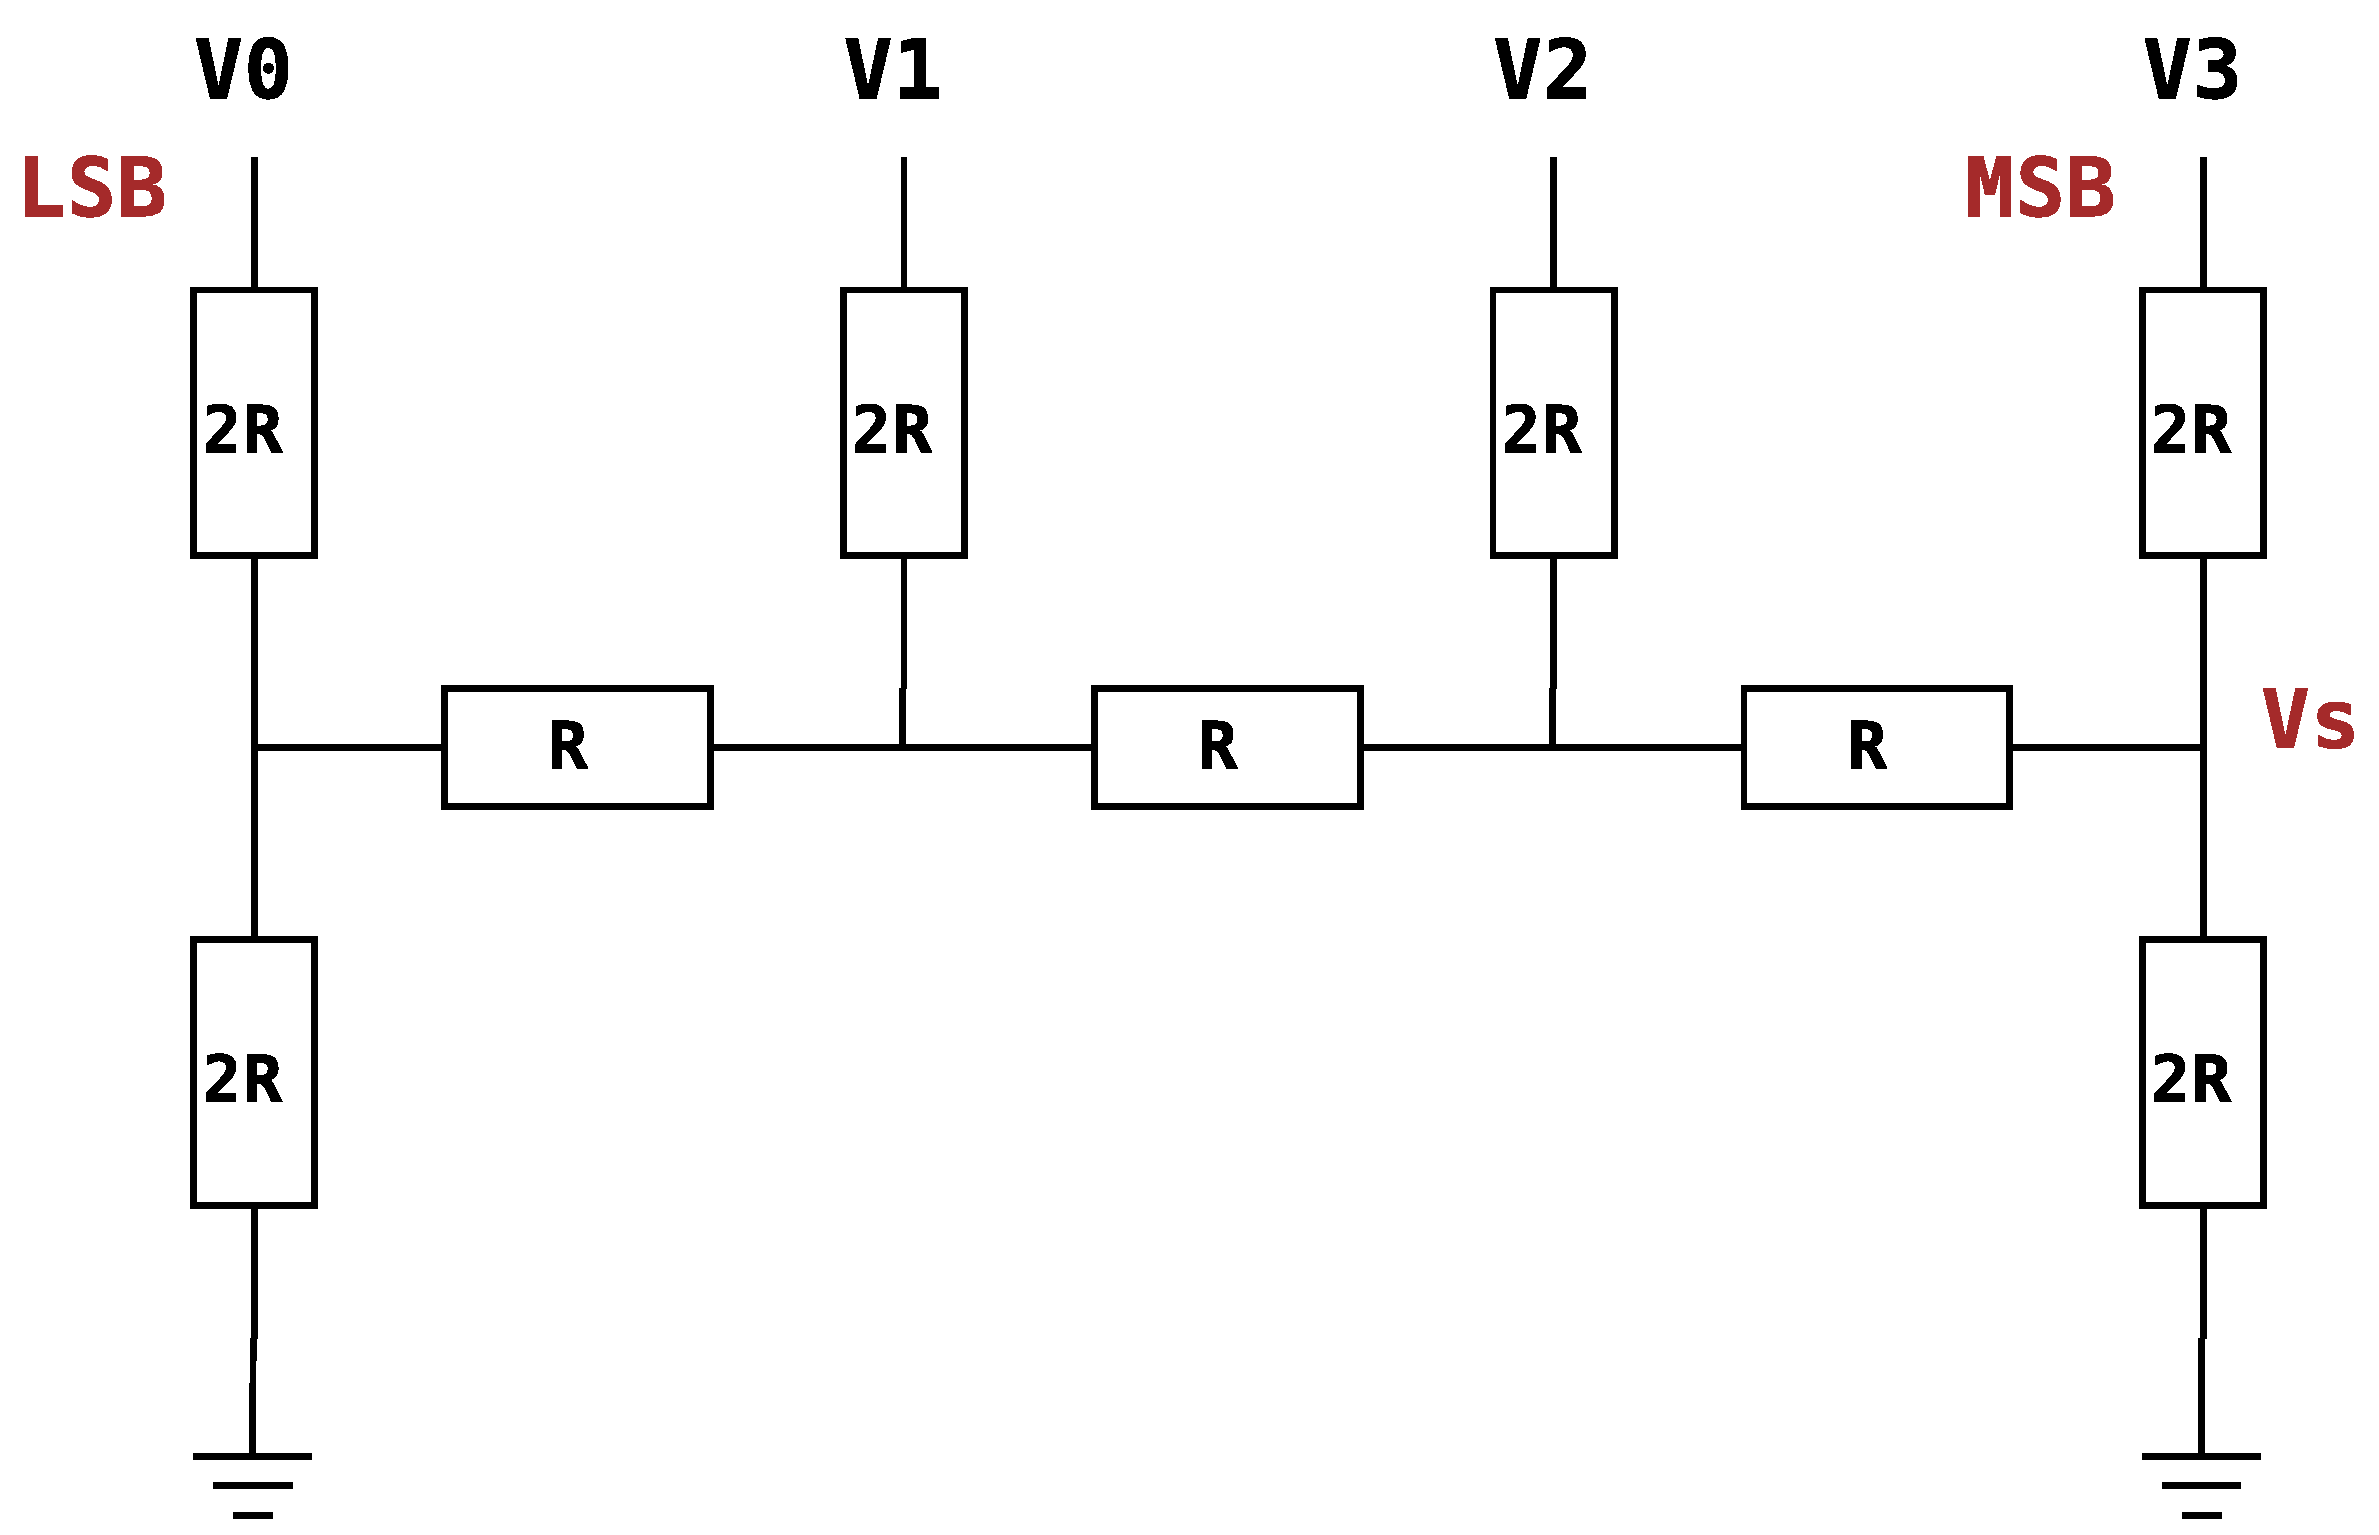
\includegraphics[width=0.6\textwidth]{images/Diagrama0.eps}
\end{center} 
\end{frame}


%%%%%%%%%%%%%%%%%%%%%%%%%%%%%%%%%%%%%%%%%%%%%%%%%%%%%%%%%%%%%%%%%%%%%%%%%%%%%%%%
\begin{frame}{Conversão digital-analógico DAC0808}
\begin{center}
\includegraphics[width=1.0\textwidth]{images/DAC0808.eps}
\end{center} 
\end{frame}
%%%%%%%%%%%%%%%%%%%%%%%%%%%%%%%%%%%%%%%%%%%%%%%%%%%%%%%%%%%%%%%%%%%%%%%%%%%%%%%%
%%%%%%%%%%%%%%%%%%%%%%%%%%%%%%%%%%%%%%%%%%%%%%%%%%%%%%%%%%%%%%%%%%%%%%%%%%%%%%%%
%%%%%%%%%%%%%%%%%%%%%%%%%%%%%%%%%%%%%%%%%%%%%%%%%%%%%%%%%%%%%%%%%%%%%%%%%%%%%%%%
\section{Conversão AD}

%%%%%%%%%%%%%%%%%%%%%%%%%%%%%%%%%%%%%%%%%%%%%%%%%%%%%%%%%%%%%%%%%%%%%%%%%%%%%%%%
% http://www.newtoncbraga.com.br/index.php/como-funciona/1508-conversores-ad
\begin{frame}{Conversão AD - Amostragem }
\begin{center}
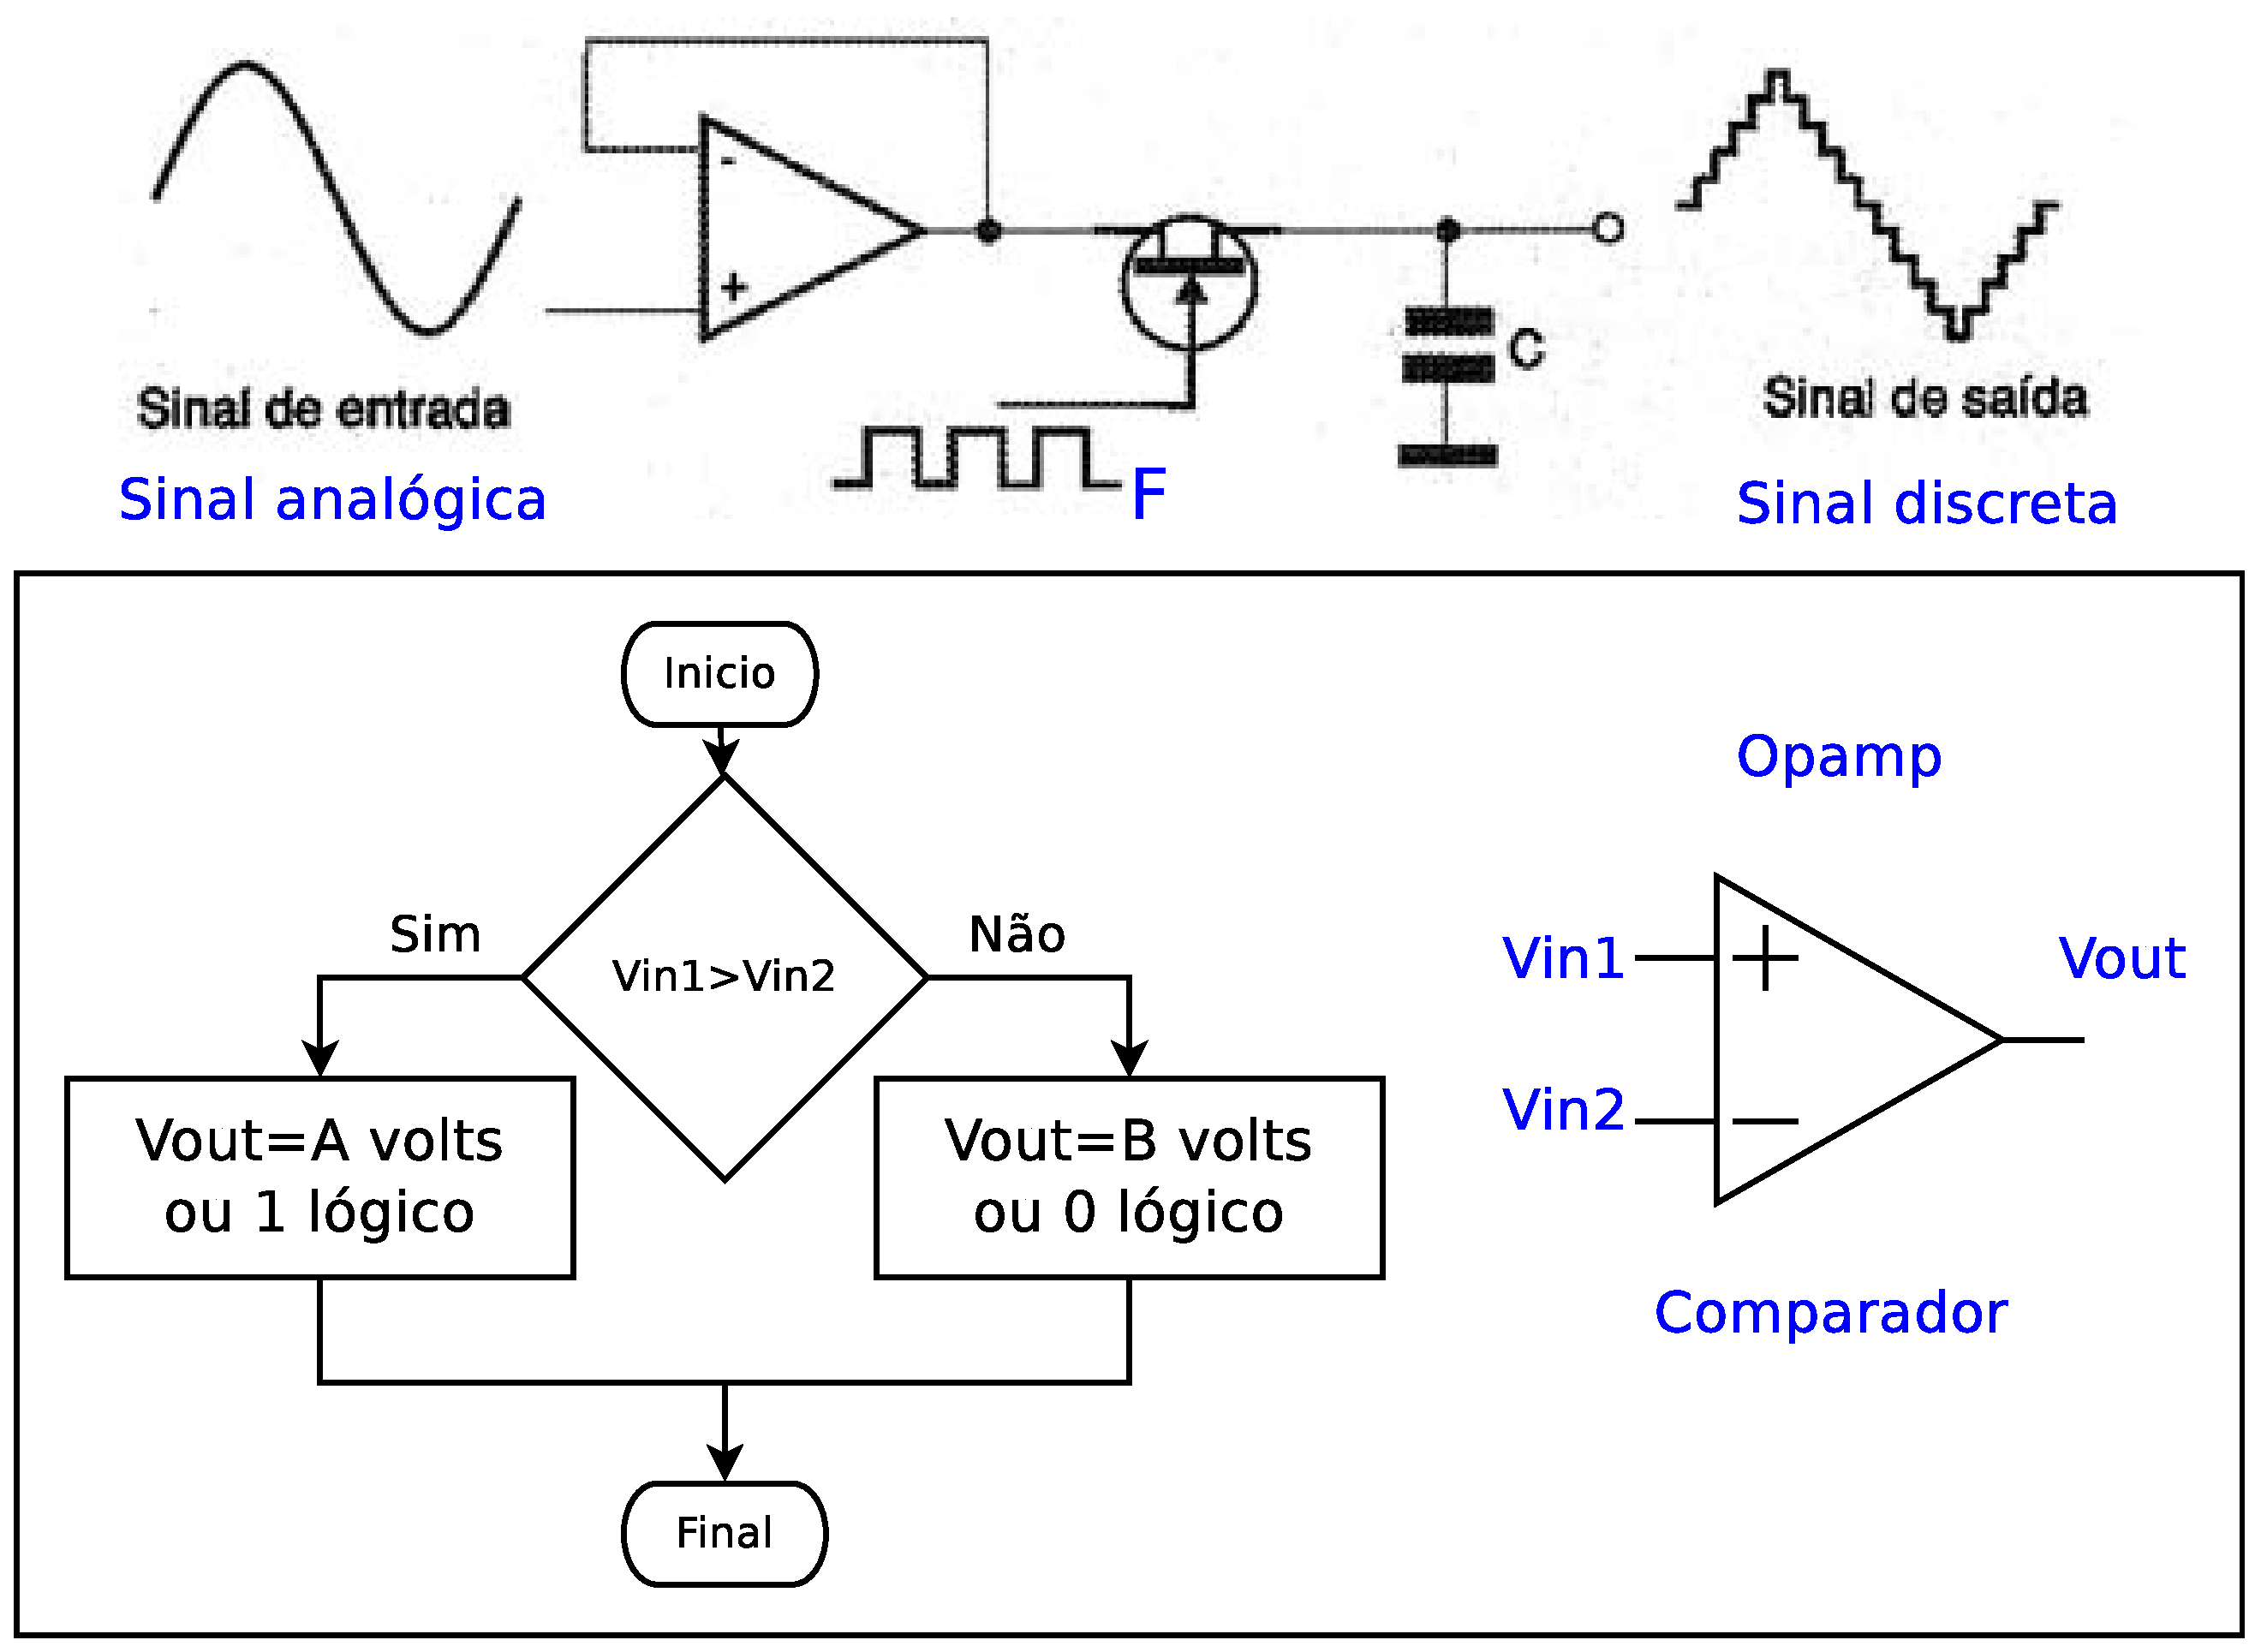
\includegraphics[width=0.8\textwidth]{images/amostragemretencao.eps}
\end{center} 
\end{frame}

%%%%%%%%%%%%%%%%%%%%%%%%%%%%%%%%%%%%%%%%%%%%%%%%%%%%%%%%%%%%%%%%%%%%%%%%%%%%%%%%
% http://www.newtoncbraga.com.br/index.php/como-funciona/1508-conversores-ad
\begin{frame}{Conversão AD simultânea (FLASH) }
\begin{center}
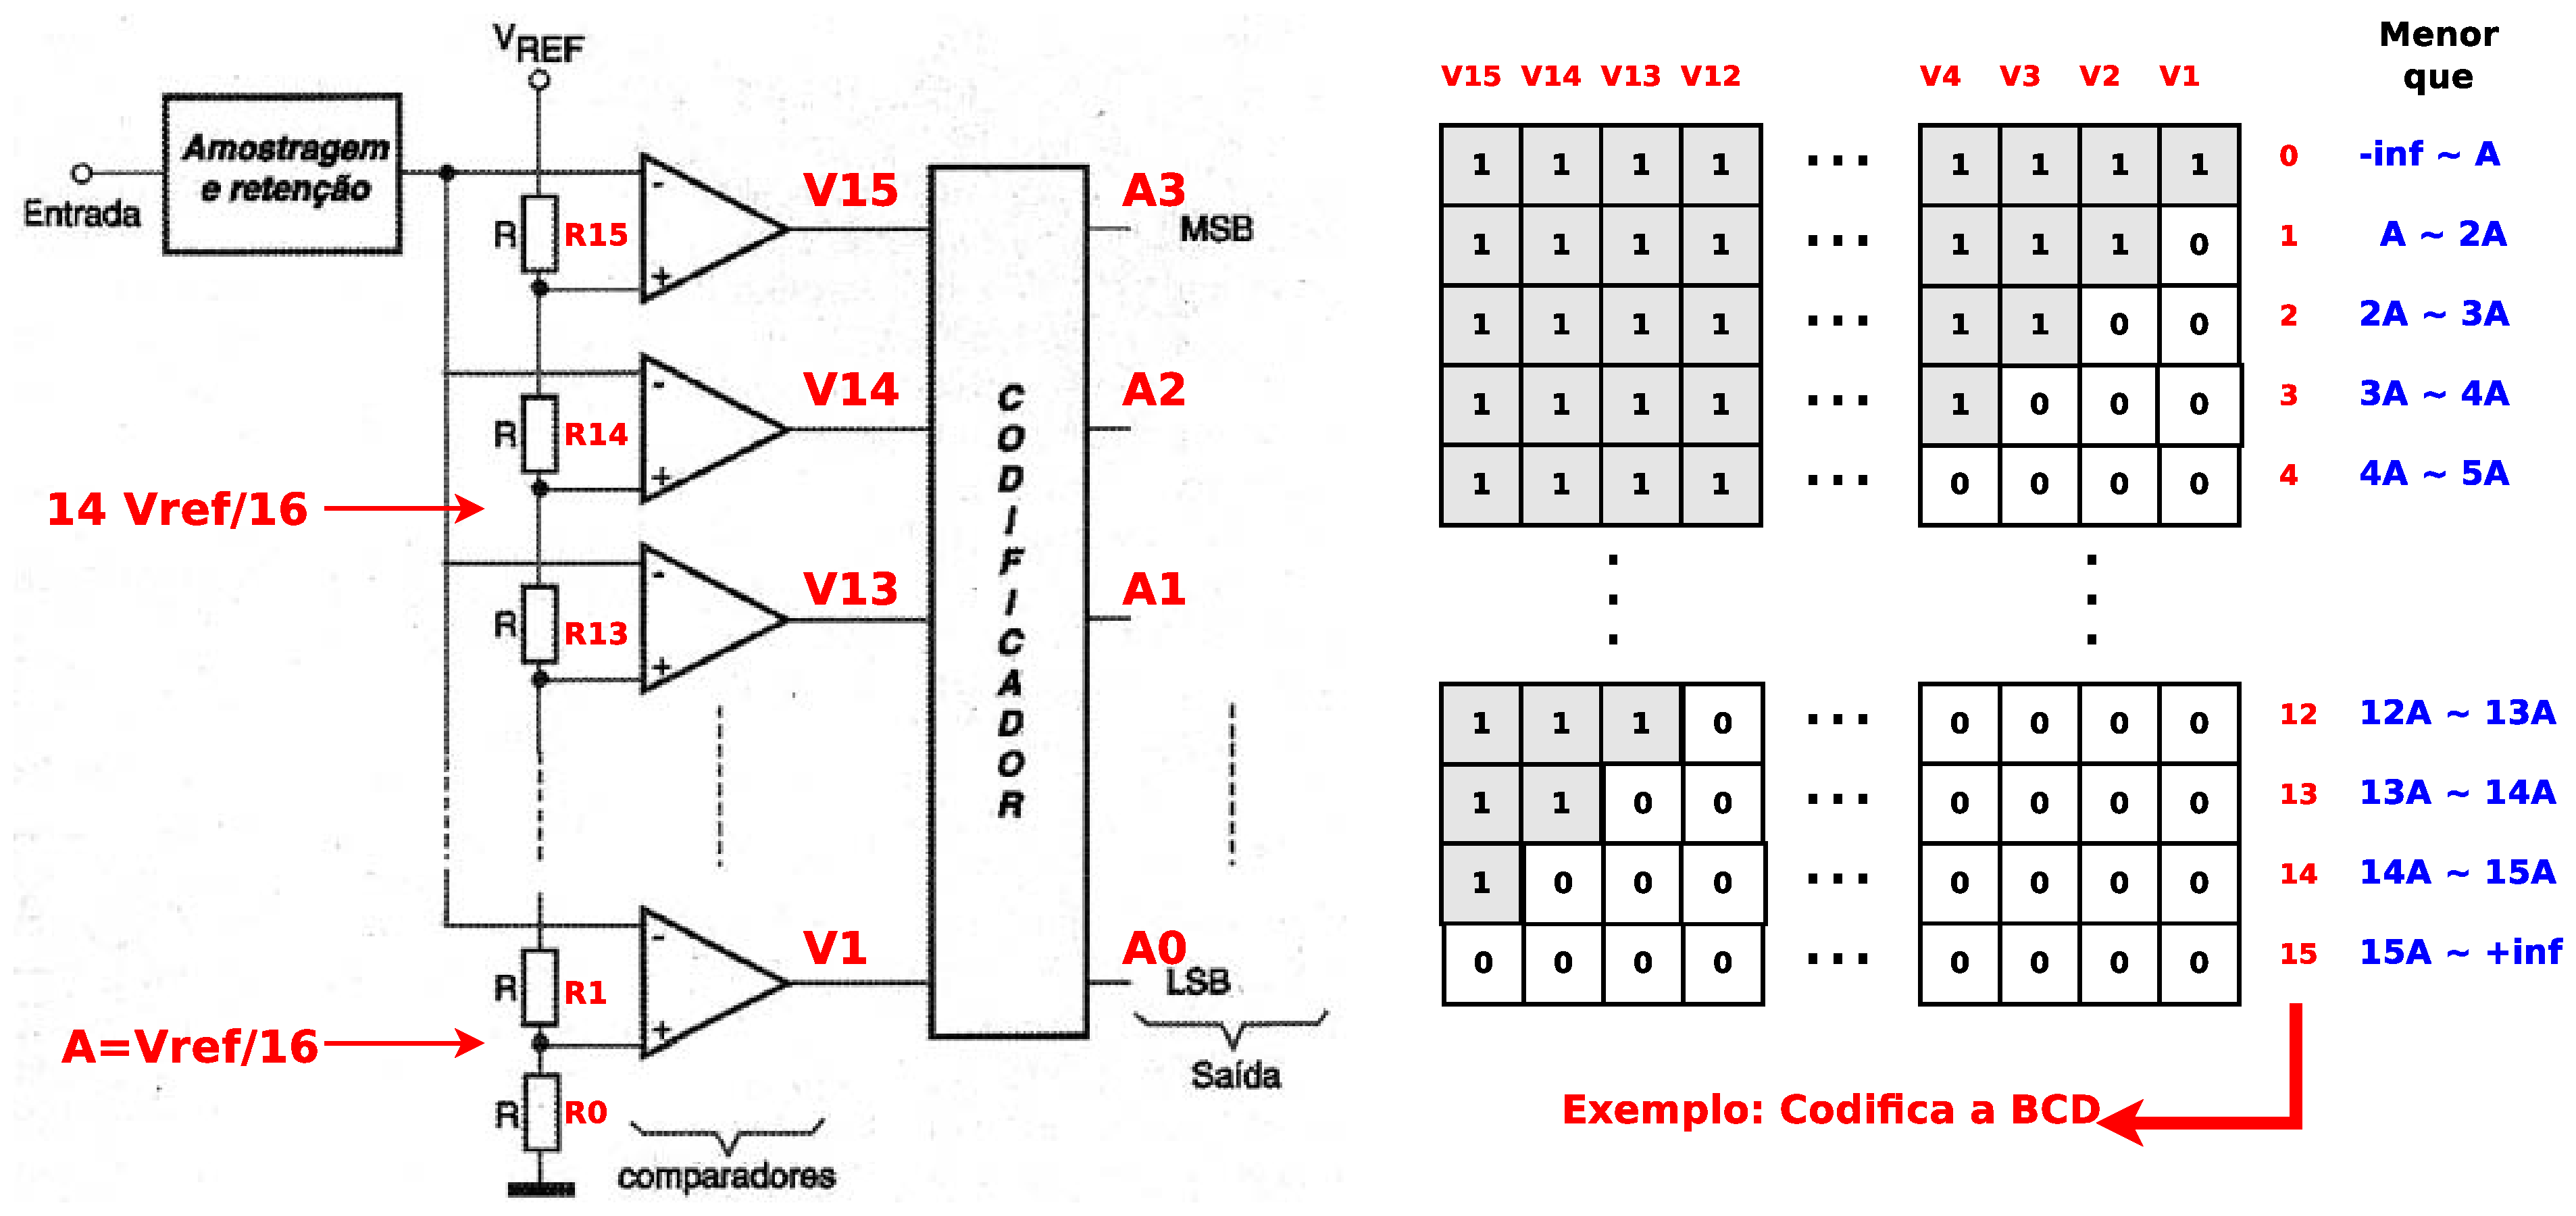
\includegraphics[width=1.0\textwidth]{images/ConversaoSimultanea.eps}
\end{center} 
\end{frame}

%%%%%%%%%%%%%%%%%%%%%%%%%%%%%%%%%%%%%%%%%%%%%%%%%%%%%%%%%%%%%%%%%%%%%%%%%%%%%%%%
% http://www.newtoncbraga.com.br/index.php/como-funciona/1508-conversores-ad
\begin{frame}{Conversão AD por contador (Rampa)}
\begin{center}
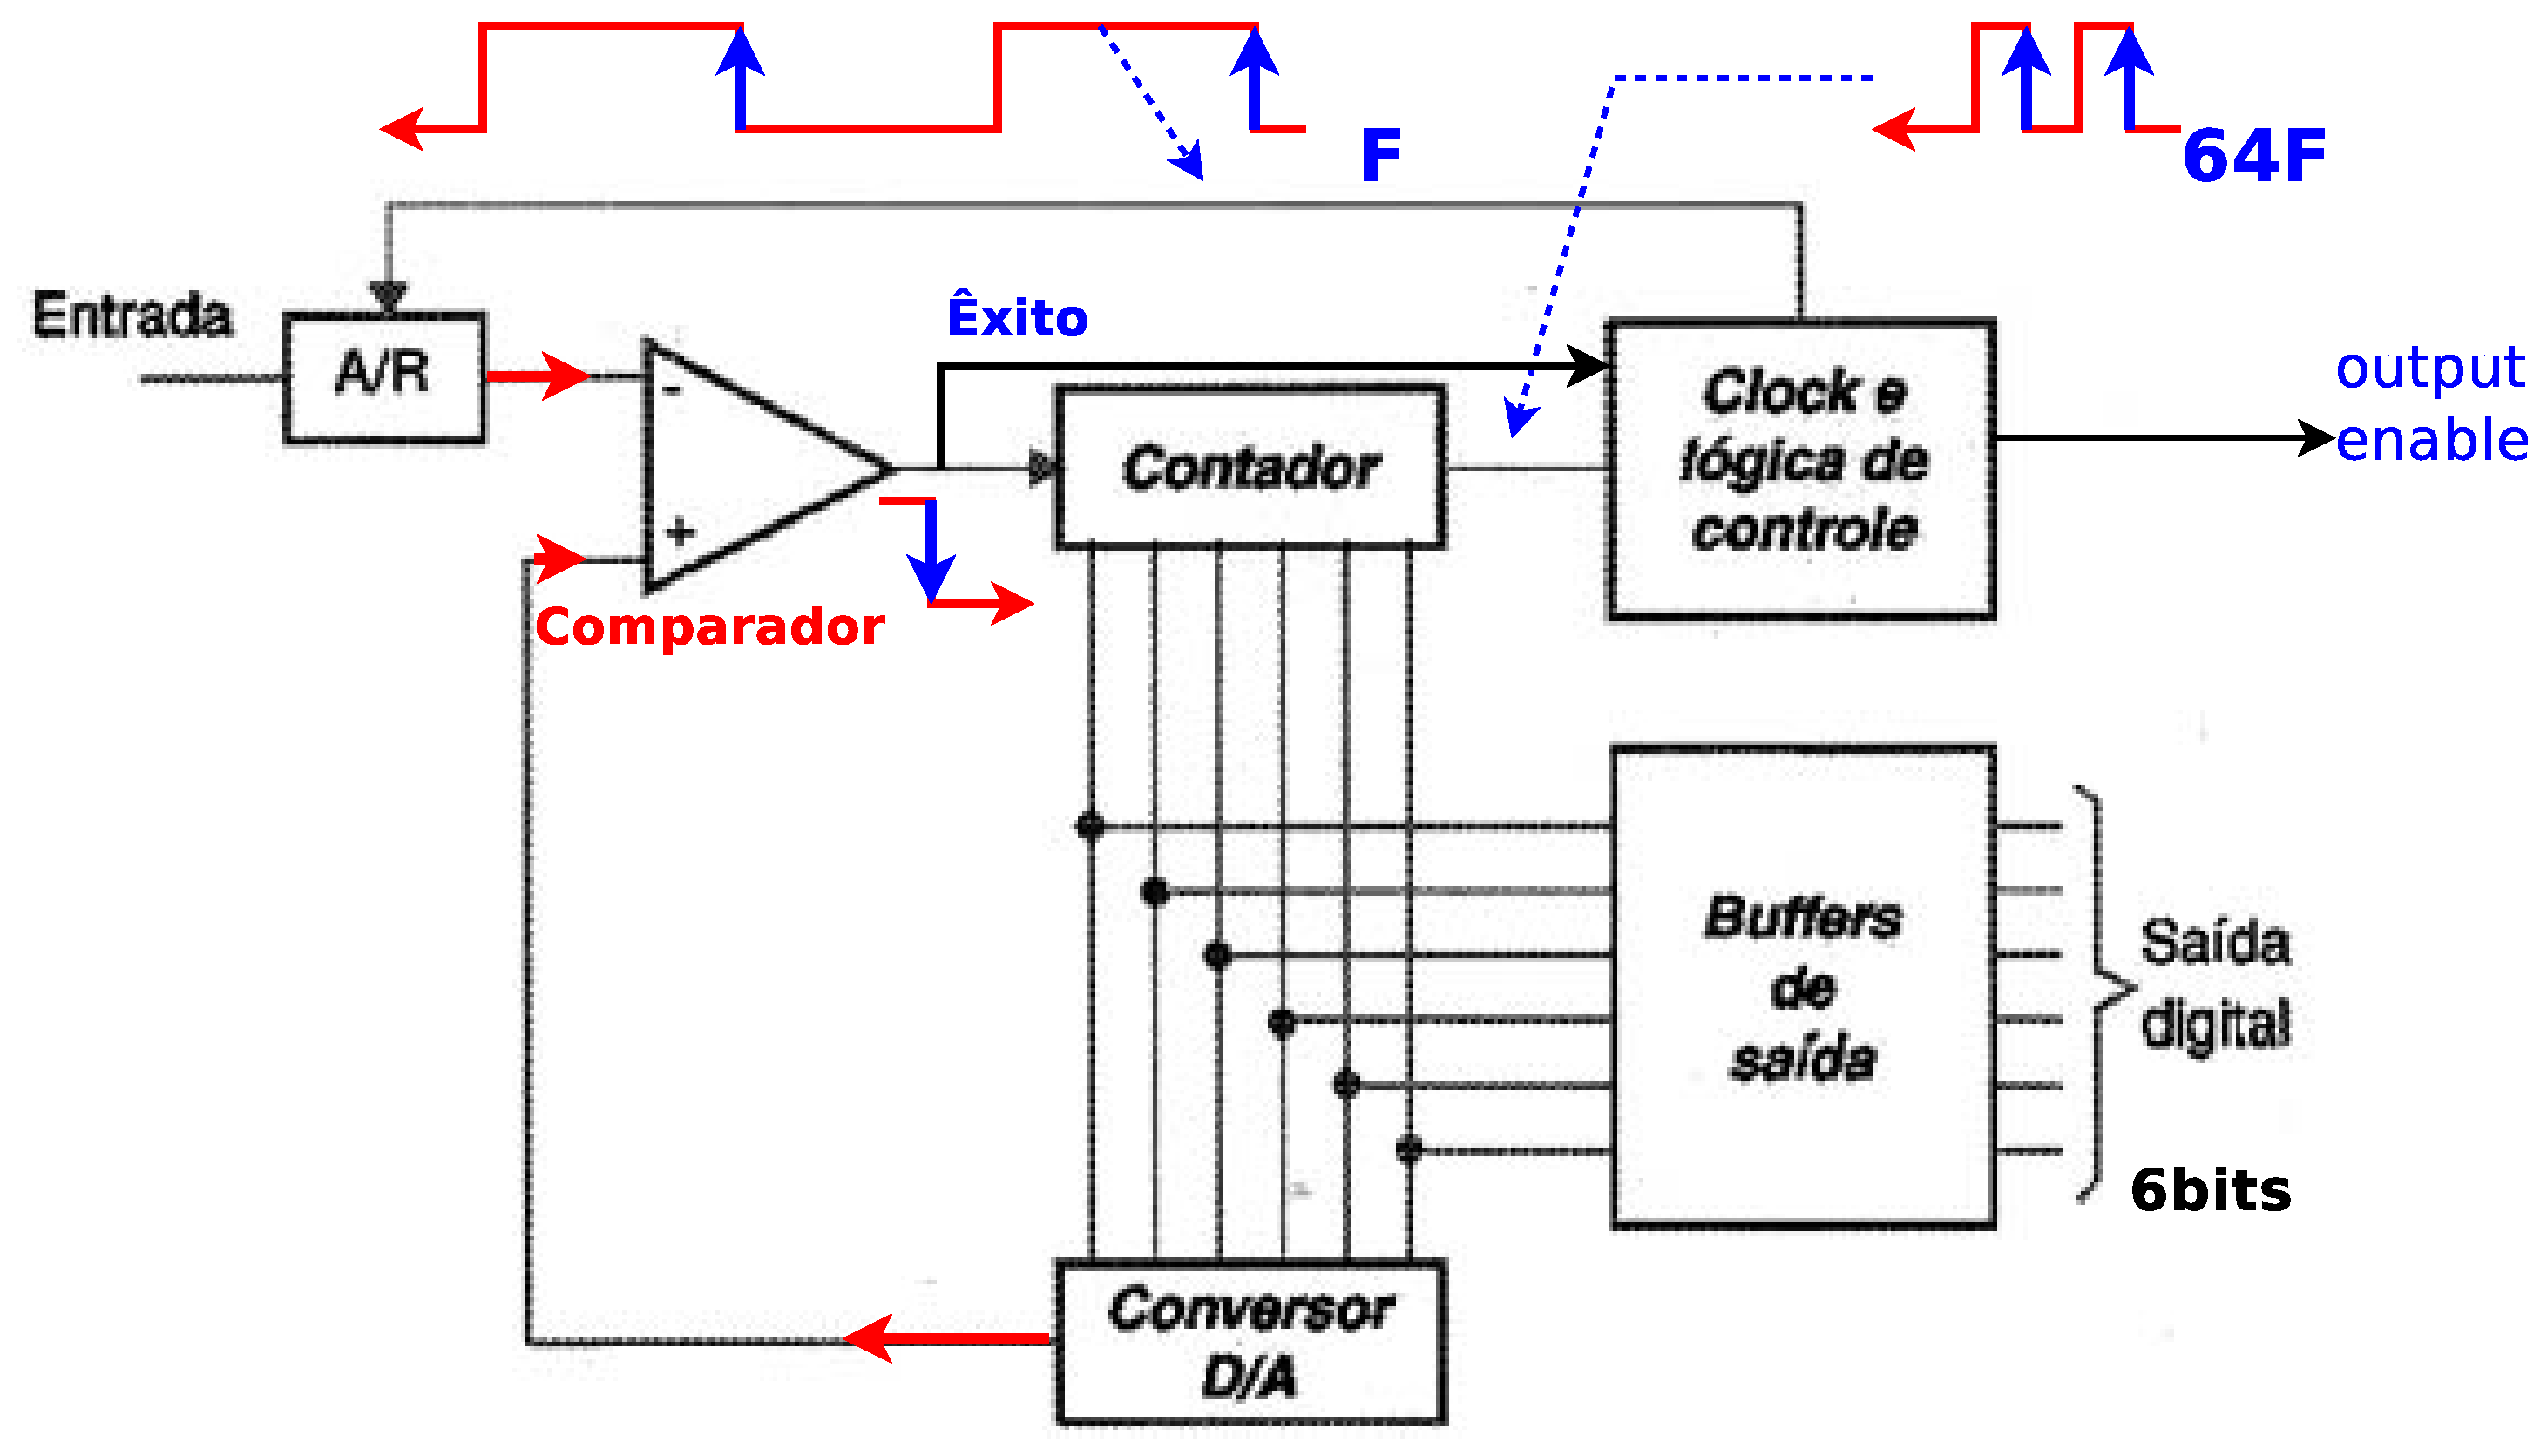
\includegraphics[width=1.0\textwidth]{images/ConversaoPorContador.eps}
\end{center} 
\end{frame}

%%%%%%%%%%%%%%%%%%%%%%%%%%%%%%%%%%%%%%%%%%%%%%%%%%%%%%%%%%%%%%%%%%%%%%%%%%%%%%%%
% http://www.ece.ufrgs.br/~fetter/ele00002/ad-da.pdf
\begin{frame}{Conversão AD por aproximações sucessivas (SAR) }
\begin{center}
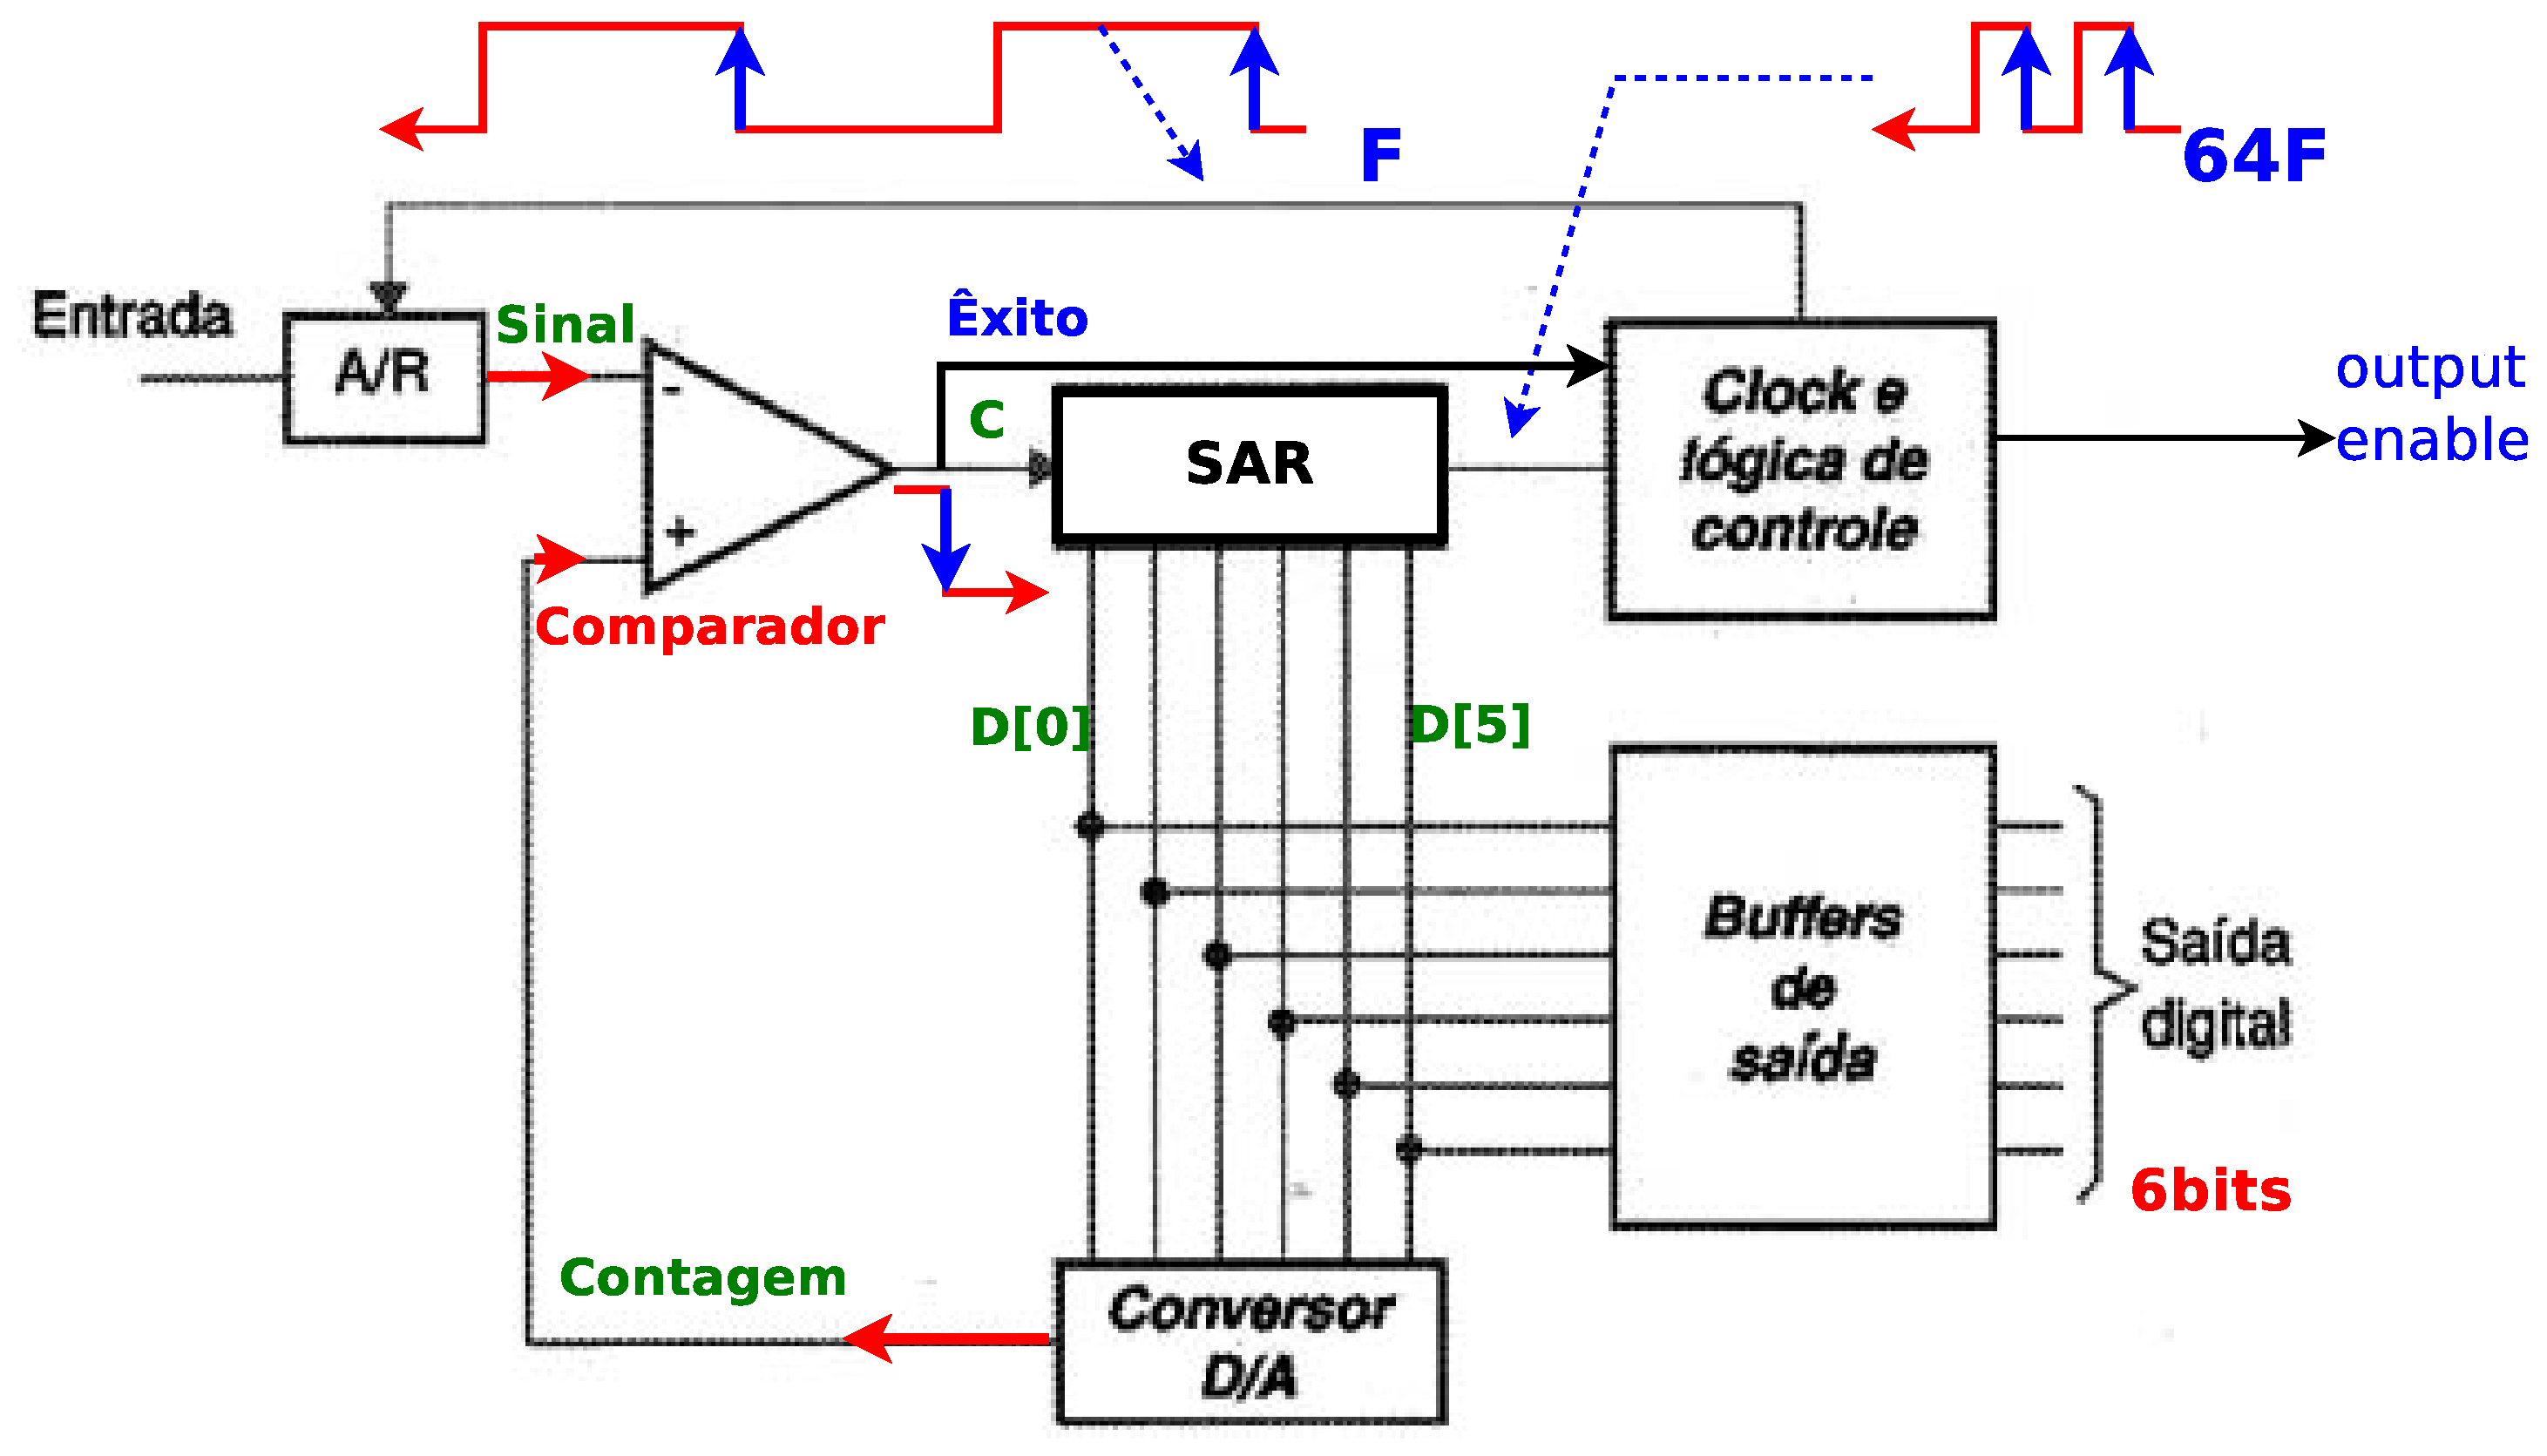
\includegraphics[width=1.0\textwidth]{images/ConversaoPorSAR.eps}
\end{center} 
\end{frame}
\begin{frame}{Conversão AD por aproximações sucessivas (SAR) }
\begin{center}
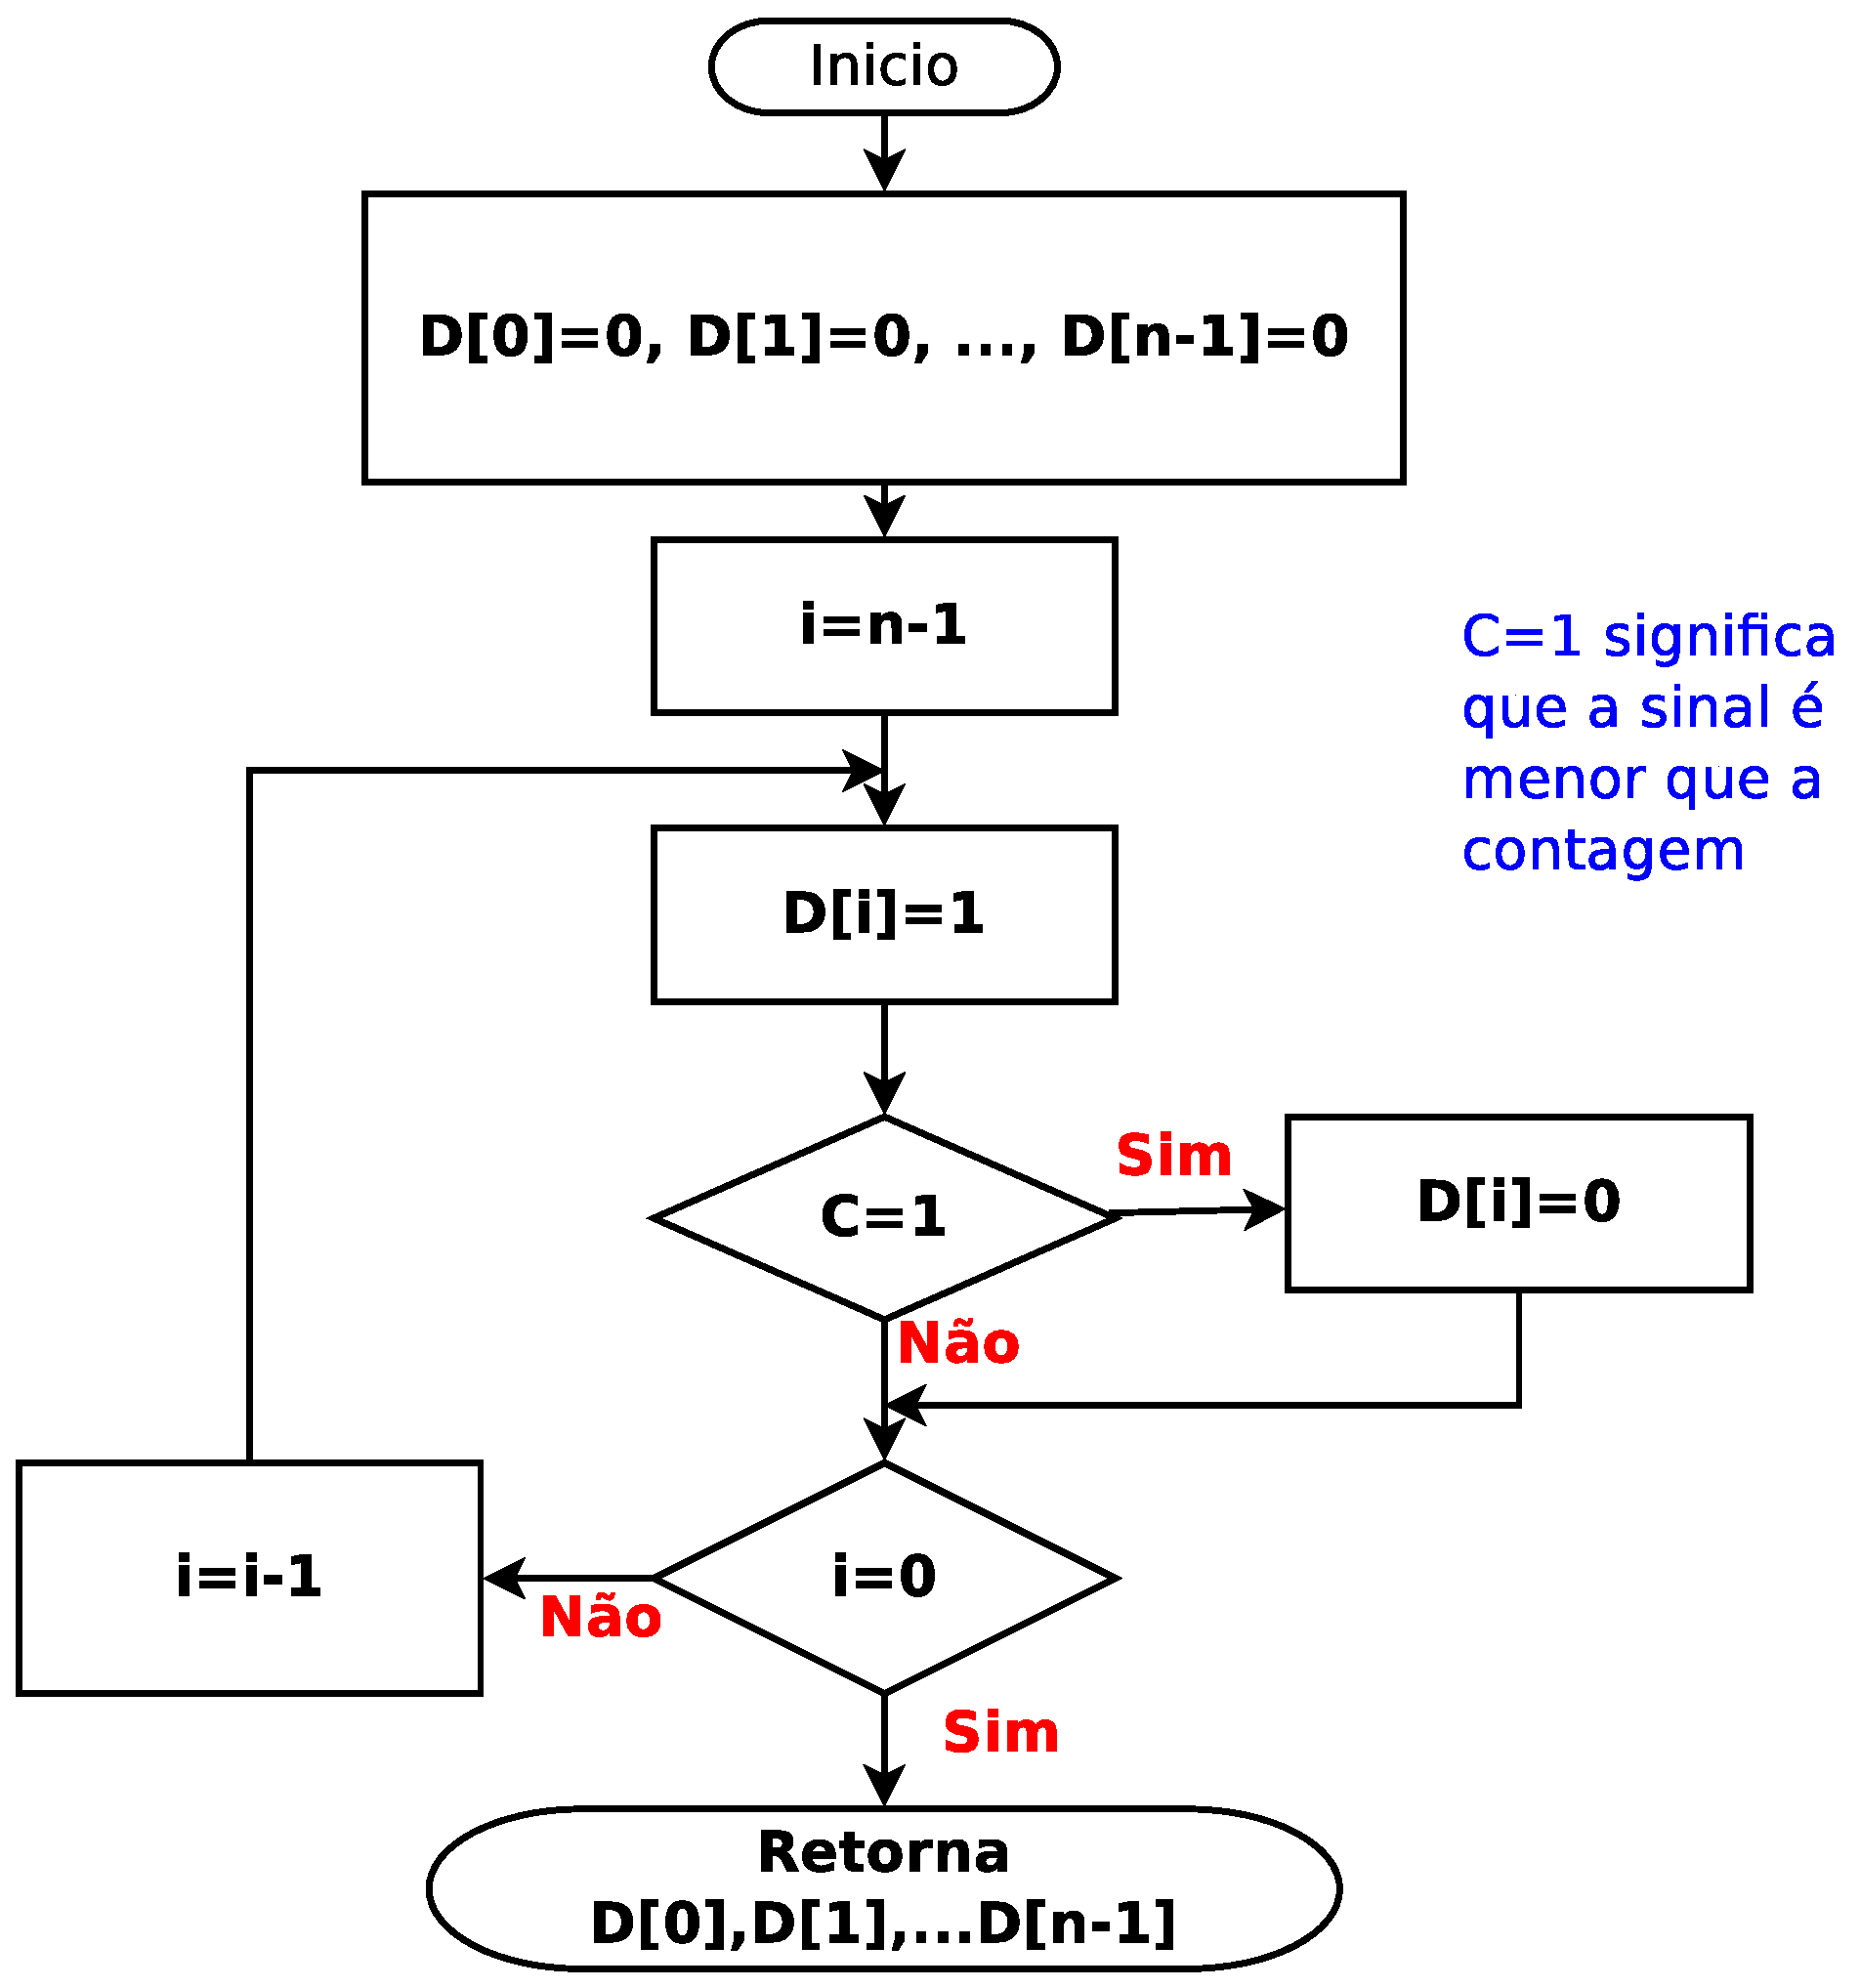
\includegraphics[width=0.5\textwidth]{images/ConversaoPorSAR2.eps}
\end{center} 
\end{frame}

%%%%%%%%%%%%%%%%%%%%%%%%%%%%%%%%%%%%%%%%%%%%%%%%%%%%%%%%%%%%%%%%%%%%%%%%%%%%%%%%
\begin{frame}{Conversão analógico-digital ADC8004}
\begin{center}
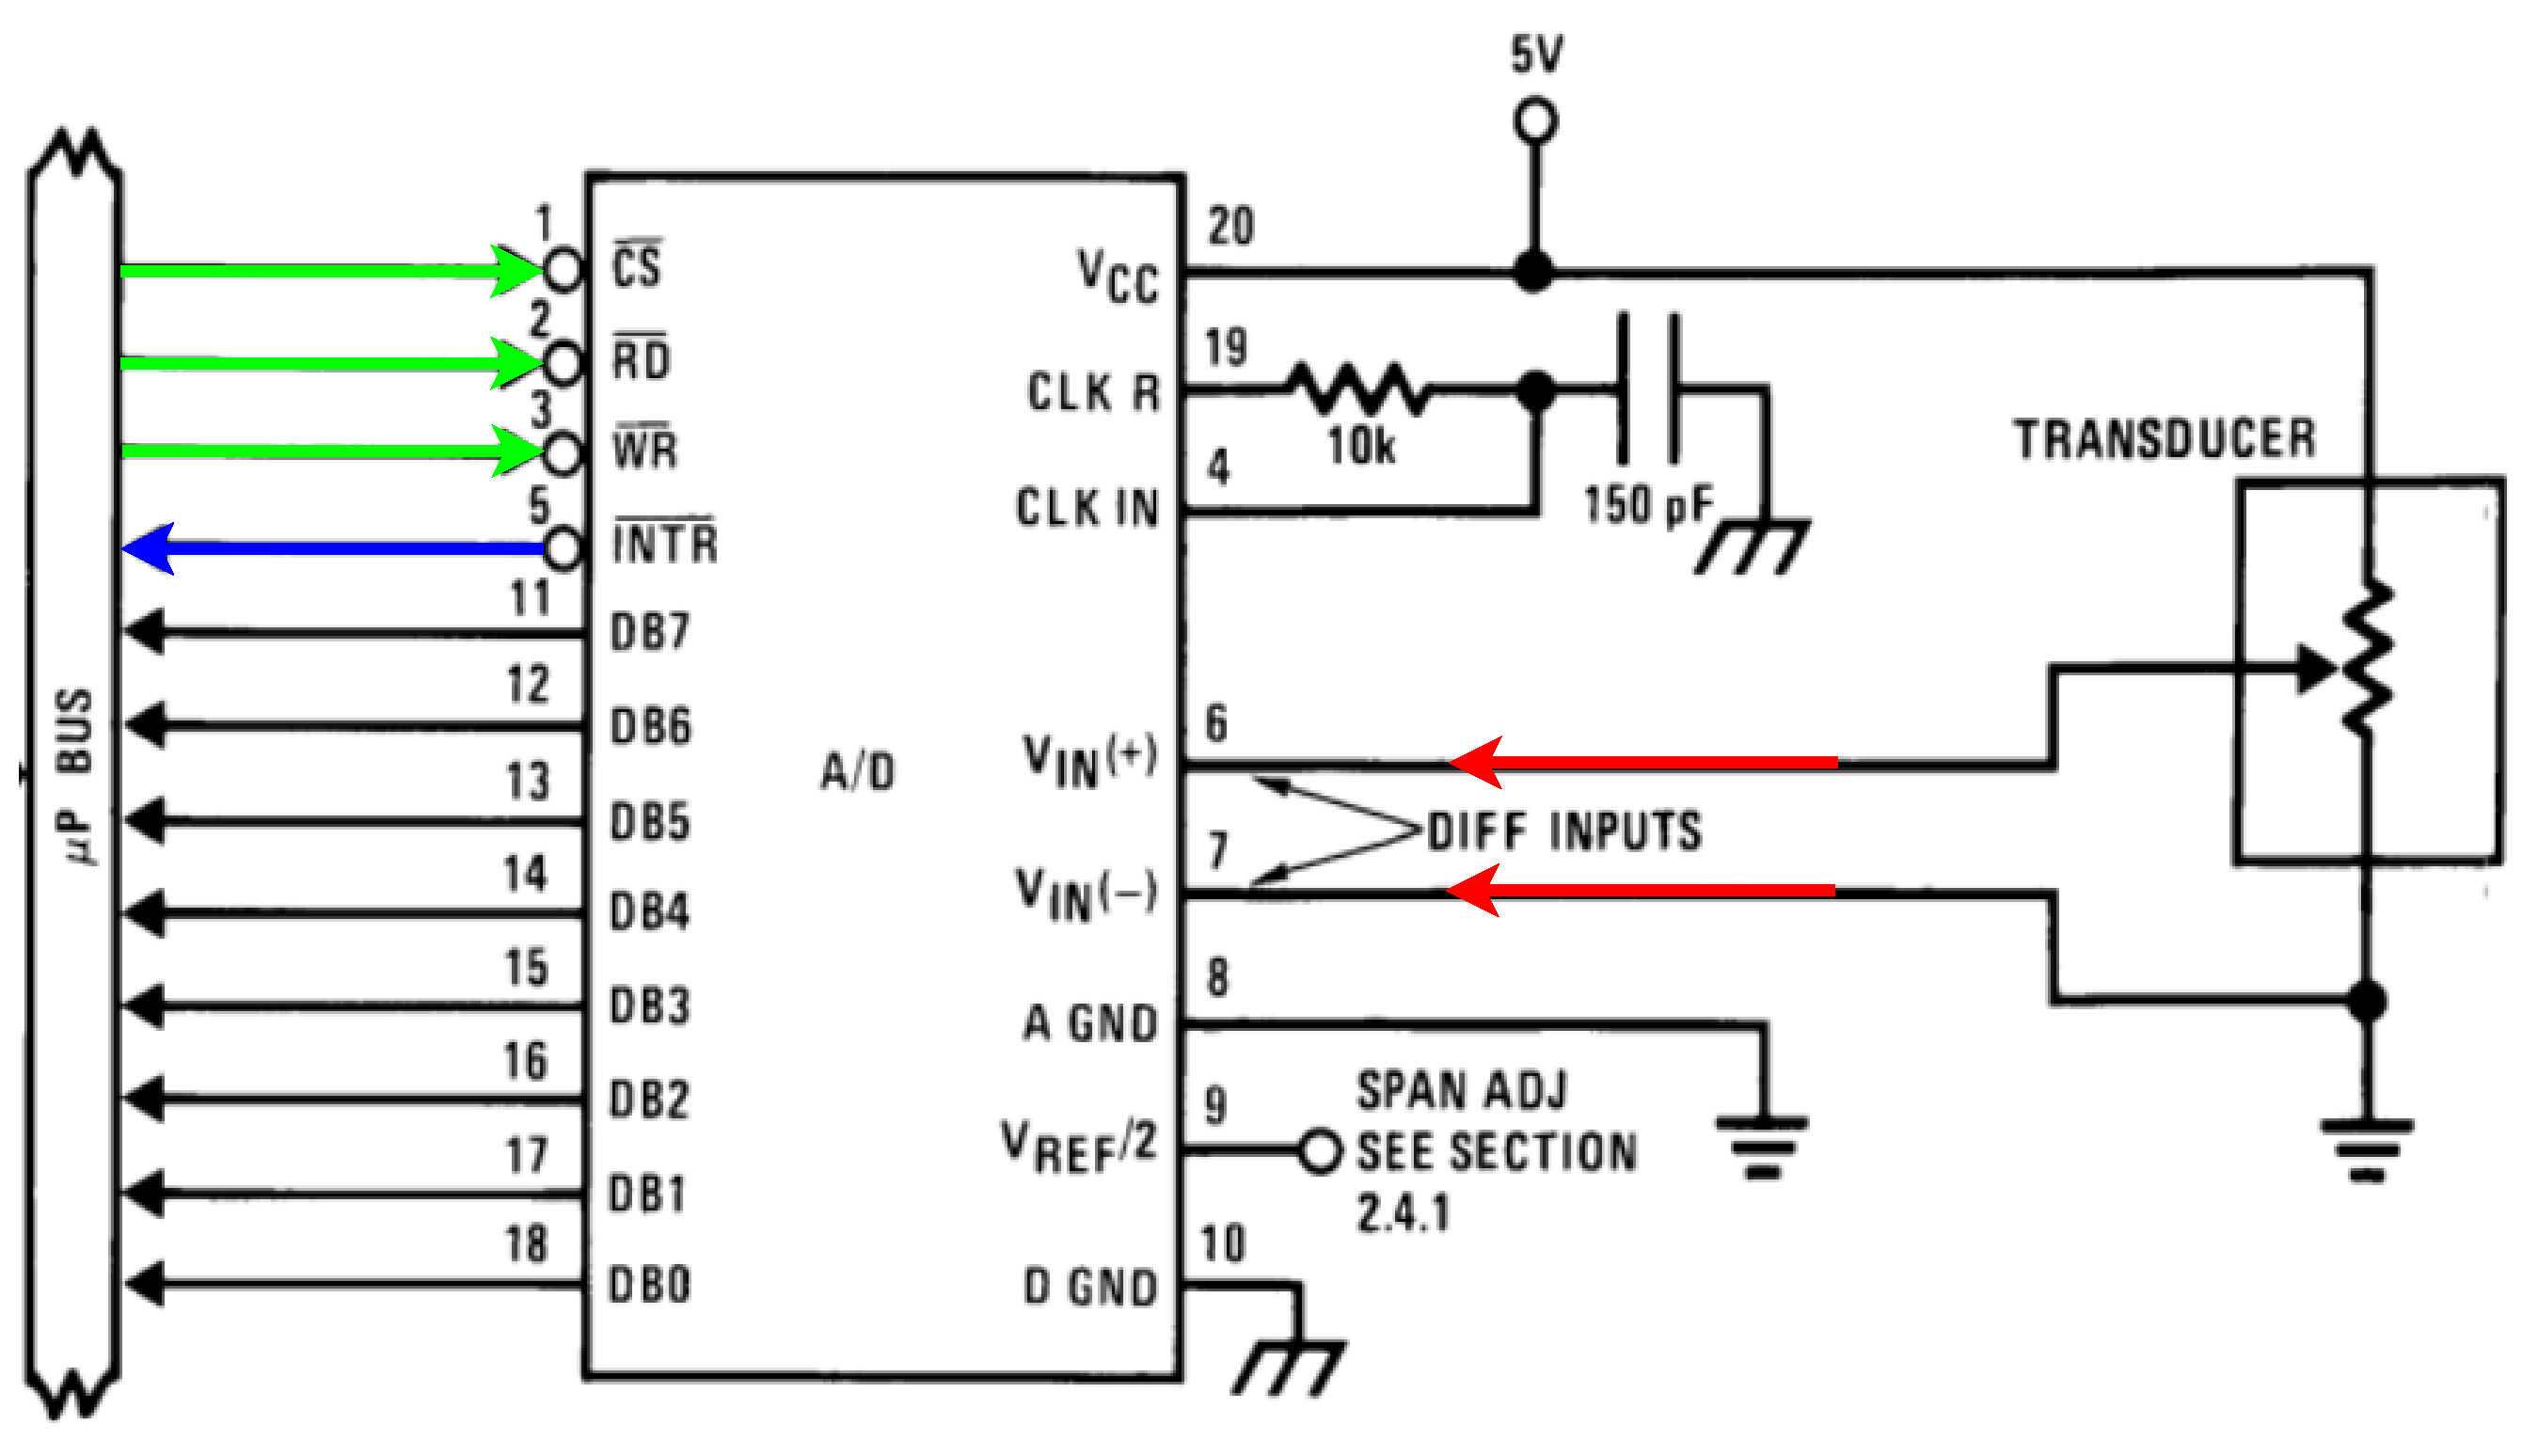
\includegraphics[width=1.0\textwidth]{images/ADC8004a.eps}
\end{center} 
\end{frame}

%%%%%%%%%%%%%%%%%%%%%%%%%%%%%%%%%%%%%%%%%%%%%%%%%%%%%%%%%%%%%%%%%%%%%%%%%%%%%%%%
\begin{frame}{Conversão analógico-digital ADC8004}
\begin{center}
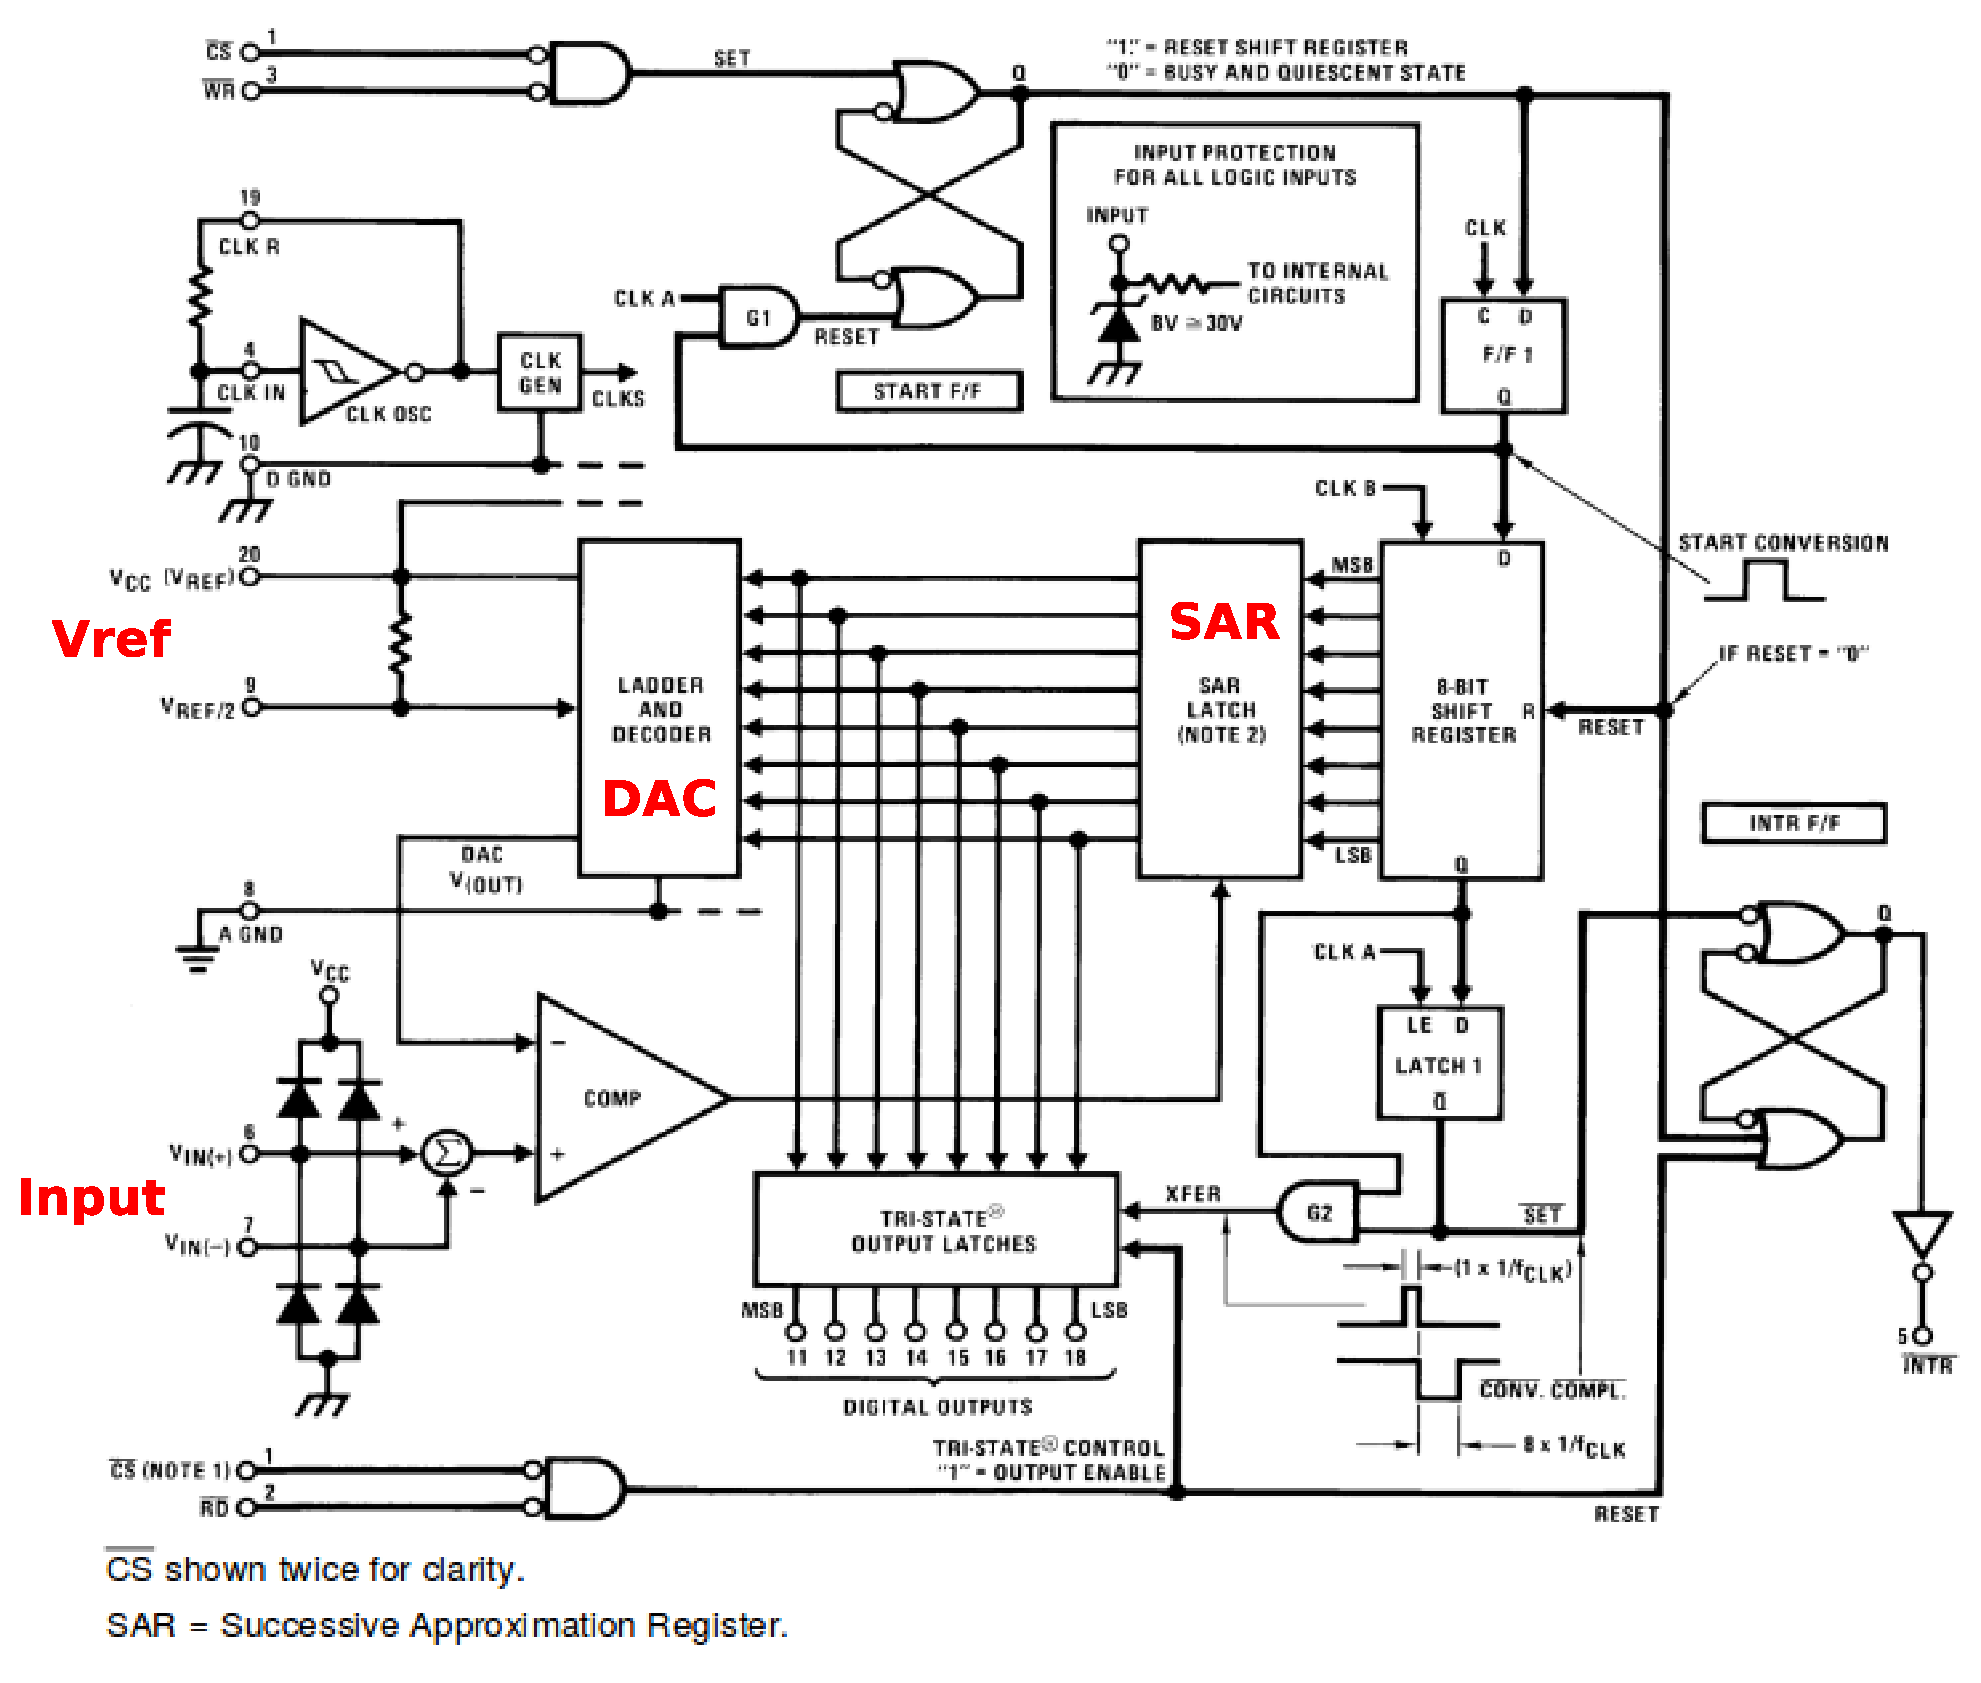
\includegraphics[width=0.7\textwidth]{images/ADC8004b.eps}
\end{center} 
\end{frame}
%%%%%%%%%%%%%%%%%%%%%%%%%%%%%%%%%%%%%%%%%%%%%%%%%%%%%%%%%%%%%%%%%%%%%%%%%%%%%%%%
\begin{frame}[allowframebreaks]
        \frametitle{References}
        \bibliographystyle{plain}
\bibliography{da-ad}
\end{frame}



\end{document}
